% Vorlage für eine Bachelorarbeit - 2012-2013 Timo Bingmann

% Dies ist nur eine Vorlage. Strikte Vorgaben wie die Bachelorarbeit auszusehen
% hat gibt es nicht. Darum können auch alle Teile angepasst werden.

% TODO: change away from the enabledeprecatedfontcommands
\documentclass[enabledeprecatedfontcommands,12pt,a4paper,twoside]{scrartcl}

% Diese (und weitere) Eingabedateien sind in UTF-8
\usepackage[utf8]{inputenc}

% Verwende gute Type 1 Font: Latin Modern
\usepackage[T1]{fontenc}
\usepackage{lmodern}

% Sprache des Dokuments (für Silbentrennung und mehr)
\usepackage[german,english]{babel}

% Seitengröße - verwende fast die ganze A4 Seite
\usepackage[tmargin=22mm,bmargin=22mm,lmargin=20mm,rmargin=20mm]{geometry}

% Einrückung und Abstand zwischen Paragraphen
\setlength\parskip{\smallskipamount}
\setlength\parindent{0pt}

% Einige Standard-Mathematik Pakete
\usepackage{latexsym,amsmath,amssymb,mathtools,textcomp}

% Unterstützung für Sätze und Definitionen
\usepackage{amsthm}

\newtheorem{Satz}{Satz}[section]
\newtheorem{Definition}[Satz]{Definition}
\newtheorem{Lemma}[Satz]{Lemma}

\numberwithin{equation}{section}

% Deutsches Literaturverzeichnis
\usepackage{bibgerm}

% Unterstützung zum Einbinden von Graphiken
\usepackage{graphicx}

% Pakete die tabular und array verbessern
\usepackage{array,multirow}

% Kleiner enumerate und itemize Umgebungen
\usepackage{enumitem}

\setlist[enumerate]{topsep=0pt}
\setlist[itemize]{topsep=0pt}
\setlist[description]{font=\normalfont,topsep=0pt}

\setlist[enumerate,1]{label=(\roman*)}

% TikZ für Graphiken in LaTeX
\usepackage{tikz}
\usetikzlibrary{calc}

% Aktuelle Section und Untersection am Seitenkopf
\usepackage{fancyhdr}

\fancypagestyle{plain}{
  \fancyhead{}
  \fancyfoot{}
  \fancyfoot[LE,RO]{\normalsize\thepage}
  \renewcommand{\headrulewidth}{0pt}
  \renewcommand{\footrulewidth}{0pt}
}

\fancypagestyle{normal}{
  \setlength{\headheight}{20pt}
  \setlength\footskip{32pt}
  \fancyhead{}
  \fancyhead[LE]{\normalsize\textsc{\nouppercase{\leftmark}}}
  \fancyhead[RO]{\normalsize\textsc{\nouppercase{\rightmark}}}
  \fancyfoot{}
  \fancyfoot[LE,RO]{\normalsize\thepage}
  \renewcommand{\headrulewidth}{0.4pt}
  \renewcommand{\footrulewidth}{0pt}
}

% Hyperref für Hyperlink und Sprungtexte
\usepackage{xcolor,hyperref}

\hypersetup{
  pdftitle={Malleable Distributed Hierarchical Planning},
  pdfauthor={Niko Wilhelm},
  pdfsubject={Stichworte, weiteres Stichwort},
  colorlinks=true,
  pdfborder={0 0 0},
  bookmarksopen=true,
  bookmarksopenlevel=1,
  bookmarksnumbered=true,
  linkcolor=blue!60!black,
  %linkcolor=black,
  citecolor=blue!60!black,
  urlcolor=blue!60!black,
  filecolor=green!60!black,
  pdfpagemode=UseNone,
  unicode=true,
}

% Paket zum Setzen von Algorithmen in Pseudocode mit kleinen Stilanpassungen
\usepackage[ruled,vlined,linesnumbered,norelsize]{algorithm2e}
\DontPrintSemicolon
\def\NlSty#1{\textnormal{\fontsize{8}{10}\selectfont{}#1}}
\SetKwSty{texttt}
\SetCommentSty{emph}
\def\listalgorithmcfname{List of Algorithms}
\def\algorithmautorefname{Algorithmus}
\let\chapter=\section % repariert ein Problem mit algorithm2e

\DeclareOldFontCommand{\bf}{\normalfont\bfseries}{\mathbf}

\usepackage{todonotes}
\usepackage{comment}
\usepackage{algorithm2e}
\usepackage{adjustbox}
\usepackage{subcaption}

\newtheorem{definition}{Definition}

\begin{document}

%%%%%%%%%%%%%%%%%%%%%%%%%%%%%%%%%%%%%%%%%%%%%%%%%%%%%%%%%%%%%%%%%%%%%%

\pagestyle{empty} % keine Seitenzahlen

% Titelblatt der Arbeit
\begin{titlepage}

  \begin{center}\large

    \quad\includegraphics[height=17mm]{kit_logo_de.pdf} \hfill
    \includegraphics[height=20mm]{grouplogo-algo-blue.pdf}\quad\null

    \vfill

    Master's Thesis
    \vspace*{2cm}

    {\bf\huge Malleable Distributed Hierarchical Planning \par}
    % Siehe auch oben die Felder pdftitle={}
    % mit \par am Ende stimmt der Zeilenabstand

    \vfill

    Niko Wilhelm

    \vspace*{15mm}

    Date of submission: \today

    \vspace*{45mm}

    \begin{tabular}{rl}
      Betreuer: & Prof. Dr. Peter Sanders \\
      & M.Sc. Dominik Schreiber \\
    \end{tabular}
    
    \vspace*{10mm}

    Institut für Theoretische Informatik, Algorithmik \\
    Fakultät für Informatik \\
    Karlsruher Institut für Technologie

    % English:
    % Institute of Theoretical Informatics, Algorithmics \\
    % Department of Informatics \\
    % Karlsruhe Institute of Technology

    \vspace*{12mm}
  \end{center}

\end{titlepage}

%%%%%%%%%%%%%%%%%%%%%%%%%%%%%%%%%%%%%%%%%%%%%%%%%%%%%%%%%%%%%%%%%%%%%%

\vspace*{0pt}\vfill

\hrule\medskip

Hiermit versichere ich, dass ich diese Arbeit selbständig verfasst und keine anderen, als die angegebenen Quellen und Hilfsmittel benutzt, die wörtlich oder inhaltlich übernommenen Stellen als solche kenntlich gemacht und die Satzung des Karlsruher Instituts für Technologie zur Sicherung guter wissenschaftlicher Praxis in der jeweils gültigen Fassung beachtet habe.

\bigskip

\noindent
Karlsruhe, den \today

% Unterschrift (handgeschrieben)

\vspace*{5cm}

\clearpage

%%%%%%%%%%%%%%%%%%%%%%%%%%%%%%%%%%%%%%%%%%%%%%%%%%%%%%%%%%%%%%%%%%%%%%

\vspace*{0pt}\vfill

\selectlanguage{german}
\begin{abstract}
\centerline{\bf Zusammenfassung}

Hier die deutsche Zusammenfassung.

Ich bin Blindtext. Von Geburt an. Es hat lange gedauert, bis ich begriffen habe, was es bedeutet, ein blinder Text zu sein: Man macht keinen Sinn. Man wirkt hier und da aus dem Zusammenhang gerissen. Oft wird man gar nicht erst gelesen. Aber bin ich deshalb ein schlechter Text? Ich weiß, dass ich nie die Chance haben werde im Stern zu erscheinen. Aber bin ich darum weniger wichtig? Ich bin blind! Aber ich bin gerne Text. Und sollten Sie mich jetzt tatsächlich zu Ende lesen, dann habe ich etwas geschafft, was den meisten ,,normalen`` Texten nicht gelingt.

Ich bin Blindtext. Von Geburt an. Es hat lange gedauert, bis ich begriffen habe, was es bedeutet, ein blinder Text zu sein: Man macht keinen Sinn. Man wirkt hier und da aus dem Zusammenhang gerissen. Oft wird man gar nicht erst gelesen. Aber bin ich deshalb ein schlechter Text? Ich weiß, dass ich nie die Chance haben werde im Stern zu erscheinen. Aber bin ich darum weniger wichtig? Ich bin blind! Aber ich bin gerne Text.

\end{abstract}

\vfill

\selectlanguage{english}
\begin{abstract}
\centerline{\bf Abstract}

And here an English translation of the German abstract.

I'm blind text. From birth. It took a long time until I realized what it means to be random text: You make no sense. You stand here and there out of context. Frequently, they do not even read. But I have a bad copy? I know that I will never have the chance of appearing in the. But I'm any less important? I'm blind! But I like to text. And you should see me now actually over, then I have accomplished something that is not possible in most ``normal'' copies.

I'm blind text. From birth. It took a long time until I realized what it means to be random text: You make no sense. You stand here and there out of context. Frequently, they do not even read. But I have a bad copy? I know that I will never have the chance of appearing in the. But I'm any less important? I'm blind! But I like to text.

\end{abstract}
%\selectlanguage{english}

\vfill\vfill\vfill
\clearpage

%%%%%%%%%%%%%%%%%%%%%%%%%%%%%%%%%%%%%%%%%%%%%%%%%%%%%%%%%%%%%%%%%%%%%%

\vspace*{0pt}\vfill

\section*{Danksagungen}
\todo{Finish!}
Thanks to my advisor, Dominik Schreiber
- ready to help me 
- the many facilities of Mallob 
Additional thanks to my friends and flatmates who helped keep me grounded during this work.
Thanks to i10pc135 which suffered much to make the experimental evaluation possible.

\vfill\vfill\vfill
\clearpage

%%%%%%%%%%%%%%%%%%%%%%%%%%%%%%%%%%%%%%%%%%%%%%%%%%%%%%%%%%%%%%%%%%%%%%

\pagestyle{normal}
% markiere sections im Seitenkopf links und subsections rechts
\renewcommand\sectionmark[1]{\markboth{\thesection\quad\MakeUppercase{#1}}{\thesection\quad\MakeUppercase{#1}}}
\renewcommand\subsectionmark[1]{\markright{\thesubsection\quad\MakeUppercase{#1}}}

% Inhaltsverzeichnis
\tableofcontents

\clearpage

%%%%%%%%%%%%%%%%%%%%%%%%%%%%%%%%%%%%%%%%%%%%%%%%%%%%%%%%%%%%%%%%%%%%%%

\listoffigures
\listoftables
\listofalgorithms

\clearpage

%%%%%%%%%%%%%%%%%%%%%%%%%%%%%%%%%%%%%%%%%%%%%%%%%%%%%%%%%%%%%%%%%%%%%%

\section{Introduction}
Planning via Hierarchical Task Networks (HTN) is a popular approach to automated AI planning. HTN planning works by repeatedly decomposing a set of initial tasks until they have been decomposed to the level of simple actions \cite{georgievski2015htn, bercher2019survey}. These actions form a plan which can be executed to achieve the goal set out by the initial tasks. Totally Ordered (TO) HTN planning is an important sub-problem of HTN planning where all tasks are constrained by a total order. \\
Hierarchical planners are easy to use as the hierarchy allows the user to insert a structure into the problem description and to provide the planner with advice to guide the planning procedure. As a result, HTN planning has been used in a number of fields. \cite{munoz2004role} have used HTN planning for AI in real-time strategy games. Similarly, \cite{ontanon2015adversarial} have improved their minimax game tree search in real-time strategy games via HTN, which allowed them to reduce the branching factor of their problem. This approach was further extended by \cite{lin2020htn} to also take the opponent's strategy into account. Further applications of HTN planning include automated web service composition \cite{sirin2004htn} as well as the composition of cloud applications \cite{georgievski2017cloud}, socially assistive robotics \cite{gonzalez2017three}, storyline visualizations \cite{padia2018yarn} and automated machine learning \cite{mohr2018ml}. \\
While popular with users, HTN planning does present challenges for implementers as instances can be very CPU and memory intensive to solve. It was shown that HTN planning itself is only semi-decidable and that TOHTN planning is still in D-EXPTIME while being EXPSPACE-hard \cite{erol1994htn, erol1996complexity}. Regarding the expressive power of TOHTN problems they correspond to the class of context-free languages \cite{holler2014language}. Part of the complexity in HTN planning stems from its recursive nature. As a result of this, the detection of duplicate states plays an important role in the performance of planners \cite{holler2021loop}. \\
\begin{comment}
- hierarchical planning is popular
- domain-independent automated planning
- decompose a set of initial tasks until they have been decomposed to the level of simple actions
- these actions form a plan which achieve the initial tasks
- TOHTN planning is a sub-problem of HTN planning where all tasks are constrained by a total order

- hierarchical planners are easy to use
- hierarchy allows the user to insert structure into the problem and advise the planner
- hierarchical planning is used in a number of domains
- \cite{munoz2004role} real-time strategy games\\
- \cite{ontanon2015adversarial} improve minimax game tree search in RTS, reduce branching factor
- \cite{lin2020htn} also takes the opponent's strategy into account

- \cite{sirin2004htn} web service composition
- \cite{georgievski2017cloud} cloud application composition

- \cite{gonzalez2017three} socially assistive robotics
- \cite{padia2018yarn} storyline visualizations
- \cite{mohr2018ml} automated machine learning

- hierarchical planning is expensive \cite{erol1994htn}
- HTN is semi-decidable, TOHTN is in D-EXPTIME, EXPSPACE-hard \cite{erol1996complexity}
- there is a correspondence between TOHTN and context free languages \cite{holler2014language}
- hierarchical problems can be recursive which makes the detection of duplicate states important
\end{comment}

Malleability is the ability of a parallel job to efficiently integrate new PEs into a parallel job at run time as well as handle a reduction of the available PEs \cite{feitelson1997job}. Malleable programs are well-liked by administrators of supercomputers, as they allow the utilization of all compute resources, maintaining both high throughput and keeping latencies for new jobs low \cite{feitelson1997job, hungershofer2004combined}. The malleable model does pose additional challenges for application programmers, though and malleable jobs are only easy to implement if we restrict our problems to those which split into small, independent work packages \cite{feitelson1997job, tucker1989process} and few malleable applications exist. 
However, in recent years a number of malleable SAT solvers have emerged. Among those Mallob \cite{sanders2022decentralized} and Paracooba \cite{heisinger2020distributed}. This is of special importance as SAT solvers serve as a building block in many other applications such as hierarchical planning. Having malleable SAT solvers available may allow for other applications to profit from this paradigm while being presented a simple to use interface. \\

In this thesis, we present three main advances in parallel and malleable TOHTN planning. \\
Firstly, we present a number of improvements for the parallel search-based planner CrowdHTN.
Both HyperTensioN \cite{magnaguagno2020hypertension} and PANDA \cite{holler2021loop} have shown the importance of detecting duplicate search nodes to improve the performance of hierarchical planners. PANDA specifically uses an approach based on hashing which may fall back to full node comparisons to avoid false positives. Parallel planner CrowdHTN already includes a loop detection mechanism based on the ideas of PANDA \cite{bretl2021parallel}. We take the idea of PANDA to only compare hashes and not full nodes and generalize it to bloom filters which may use any number $k$ of hash functions to reduce false positive rates. Bloom filters then allow us to present a design for a distributed loop detection mechanism. Additionally, PANDA has shown that heuristics can greatly increase the performance of search-based planner \cite{holler2020htn}. We try to adapt heuristic search for CrowdHTN while under the added constraints of malleability. Doing so, we implement BFS, heuristic DFS and A-star in CrowdHTN.
Last, we take inspiration from SAT where restarts have been used since the 90's \cite{crawford1994experimental} to design a restarting scheme for CrowdHTN which allows it to be complete even as bloom filter based detection of duplicate nodes may lead to false positives. \\
Second, we provide a general overview of the completeness of different TOHTN planning approaches. We show that both search-based planners using BFS, A-star and current SAT-based planners are complete. In addition we argue that heuristic best-first search may always be incomplete and that, while current loop detection mechanisms are helpful for planner performance, there are cases of recursion in hierarchical planning problems which they are unable to detect. Lastly, we show that our restart mechanism brings random DFS into the list of algorithms which are complete on all problems. \\
Third, we present our design of a malleable TOHTN planner. In this we integrate our planner CrowdHTN with the malleable job scheduler Mallob. We offer an overview of our design and show how work stealing in general can be adapted to a malleable framework while preserving completeness of the search. Doing so we also show Mallob's capabilities as a general purpose job scheduler and load balancer.\\
In our evaluation we find that our implementation suffers from some overhead due to the integration into the Mallob scheduler.
However, we also see that bloom filters in general outperform hash sets when it comes to detecting duplicate states in TOHTN planning and that this performance gain extends to our distributed loop detection scheme. We further find that restarts not only serve to ensure the completeness of our planner while using bloom filters but have an additional positive impact on overall performance. Regarding malleability, we see that our proposed malleable work stealing scheme can suffer from some loss of performance when a large number of PEs is frequently reshuffled but that this can be mitigated with frequent restarts. \\

The rest of this work follows the following structure: in section \ref{prelim} we introduce a TOHTN planning formalism as well as planning techniques, followed by an intro to malleability and an overview of parallel and distributed computing techniques that inform the design of CrowdHTN. It ends with a short introduction to CrowdHTN and Mallob. Section \ref{improv} presents us two potential theoretical improvements to CrowdHTN and the design of a distributed loop detection scheme. In section \ref{improv: completeness} we show how current loop detection schemes are unequipped to ensure completeness of hierarchical planners and argue for the use of restarts as an alternative technique. Section \ref{malleable: overview} presents our design of a malleable parallel TOHTN planner based on work stealing. This is followed by section \ref{impl} which contains implementation details of both our improvements and the malleable design. Finally, section \ref{eval} evaluates and compares our planner to it's old standalone version, presents the performance impact of our various improvements and provides an overview of the behavior of CrowdHTN as the number of PEs scales as well as under malleable conditions. Section \ref{conclusion} concludes this work.
	
\clearpage
\pagebreak
\section{Preliminaries}
\label{prelim}
\subsection{(TO)HTN Formalism}
\label{prelim: formalism}
In this section we first define what HTN and TOHTN problems are from a formal perspective \ref{prelim: tohtn problems}. Afterwards we take a short look at the algorithmic worst case complexity of HTN and TOHTN planning \ref{prelim: tohtn complexity}. We conclude by taking a short look at how hierarchical and classical planning compare in \ref{prelim: planning differences} and present the way in which we visualize hierarchical problems in this work in \ref{prelim: graphic tohtn}.

\subsubsection{Defining (TO)HTN Planning Problems}
\label{prelim: tohtn problems}
Both HTN and TOHTN planning are based on decomposing a list of initial tasks down into smaller subtasks until those subtasks can be achieved by simple actions. A number of formalisms for HTN plannings exist \cite{georgievski2015htn, behnke2018tracking, schreiber2021lilotane}. These formalisms are similar but differ slightly to suit specific planning approaches. In this work, we will reuse the formalism we introduced in \cite{bretl2021parallel} which is built on the definition by \cite{georgievski2015htn}.

\begin{definition} % predicate
	A \textbf{predicate} consists of two parts. Firstly a predicate symbol $p \in \mathcal{P}$ where $\mathcal{P}$ is the finite set of predicate symbols. Secondly of a list of terms $\tau_1, \ldots, \tau_k$ where each term $\tau_i$ is either a constant symbol $c \in \mathcal{C}$, with $\mathcal{C}$ being the finite set of constant symbols, or a variable symbol $v \in \mathcal{V}$, where $\mathcal{V}$ is the infinite set of variable symbols. \\
	The set of all predicates is called $\mathcal{Q}$.
\end{definition}
With the definition of a predicate in place, we can then define a grounding as well as our world state.
\begin{definition} % grounding
	A \textbf{ground predicate} is a predicate where the terms contain no variable symbols or, in other words, a predicate that contains only constant symbols.
\end{definition}
\begin{definition} % state
	A \textbf{state} $s \in 2^{\mathcal{Q}}$ is a set of ground predicates for which we make the closed-world-assumption. Under the closed-world-assumption, only positive predicates are explicitly represented in $s$. All predicates not in $s$ are implicitly negative.
\end{definition}

\begin{definition} % primitive task/ action
	With $T_p$ the set of primitive task symbols, a \textbf{primitive task} $t_p$ is defined as a triple $t_p(\Tilde{t}_p (a_1, \ldots, a_k), pre(t_p), eff(t_p))$. $\Tilde{p} \in T_p$ is the task symbol, $a_1, \ldots, a_k \in \mathcal{C} \cup \mathcal{V}$ are the task arguments, $pre(t_p) \in 2^{\mathcal{P}}$ the preconditions and $eff(t_p) \in 2^{\mathcal{P}}$ the effects of the primitive task $t_p$. We further define the positive and negative preconditions of $t_p$ as $pre^+(t_p) := \{p \in pre(t_p) : p \text{ is positive}\}$ and $pre^-(t_p) := \{p \in pre(t_p) : p \text{ is negative}\}$. We define $eff^+(t_p)$ and $eff^-(t_p)$ analogously. \\
	We call a fully ground primitive task an \textbf{action}.
\end{definition}

As preconditions and effects may not be concerned with the whole world state the closed-world assumption does not apply to them. To any HTN instance we could create an equivalent one where each precondition and effect cares about the whole world state. This would be achieved by instantiating all the "don't care" terms in preconditions and effects with all possible combinations of predicates. Doing this would, however, come at the price of a huge blowup of our planning problem. \\

\begin{definition} % applicable, application
	An action $t_p$ is \textbf{applicable} in state $s$ if $pre^+(t_p) \subseteq s$ and $pre^-(t_p) \cap s = \emptyset$. The \textbf{application} of $t_p$ in state $s$ results in the new state $s' = (s \setminus eff^-(t_p)) \cup eff^+(t_p)$.
\end{definition}

\begin{definition} % compound task/ abstract task
	We define a \textbf{compound task} as $t_c = \Tilde{t}_c(a_1, \ldots, a_k)$, where $\Tilde{t_c} \in T_c$ is the task symbol from the finite set of compound task symbols $T_c$ and $a_1, \ldots, a_k$ are the task arguments.
\end{definition}
Primitive and compound tasks together form task networks. In places where both can be used, we will refer to them simply as tasks $t \in T$.

\begin{definition} % task network
	Let $T = T_p \bigcup T_c$ be a set of primitive and compound tasks. A task network is a tuple $\tau = (T, \psi)$ consisting of tasks $T$ and constraints $\psi$ between those tasks.
\end{definition}

\begin{definition} % method, reduction
	Let $M$ be a finite set of method symbols and $T = T_p \bigcup T_c$ a set of primitive and compound tasks. A \textbf{method} $m = (\Tilde{m}(a_1, \ldots, a_k), t_c, pre(m), subtasks(m), constraints(m))$ is a tuple consisting of the method symbol $\Tilde{m}$, the method arguments $a_1, \ldots, a_k$, the associated compound task $t_c \in T_c$ the method refers to, a set of preconditions $pre(m) \in 2^{\mathcal{P}}$, a set of tasks $subtasks(m) = \{t_1, \ldots, t_l\}, t_i \in T$ and a set of ordering constraints $c_1, \ldots, c_m$ defining relationships between the subtasks. Any arguments appearing in $t_c, pre(m), subtasks(m)$ must also appear in $a_1, \ldots, a_k$.\\
	In TOHTN planning, $constraints(m)$ is implicitly set s.t. the subtasks $t_1, \ldots, t_l$ are totally ordered. \\
	We call a fully ground method a \textbf{reduction}.
\end{definition}
Each method $m$ has exactly one associated compound task $t_c$. However, multiple methods $m_1, \ldots, m_k$ may be associated with a single compound task $t_c$. Additionally, while any arguments of $t_c$ must be present in $m$, the contrary is not true and $m$ may have arguments not present in $t_c$, i.e., $m$ is not fully determined by $t_c$. As a result, methods represent choice points both in the choice of method itself as well as through the argument instantiation. \\


\begin{definition} % resolving a compound task
	Let $\tau = (T, \psi)$ be a task network, $s$ a state, $m = (\Tilde(m)(a_1, \ldots, a_k), t_c, pre(m),$\\$ subtasks(m), constraints(m))$ be a method. $m$ \textbf{resolves} $\tau$ iff $t_c \in T$, the constraints in $\psi$ allow for $t_c$ to be resolved, $pre^+(m) \in s$ and $pre^-(m) \cap s = \emptyset$. \\
	Resolving a compound task $t \in T$ results in a new task network $\tau' = ((T \setminus t) \cup \{t : t \in subtasks(m)\}, \psi \cup constraints(m))$ and unchanged state $s$. \\
	Applying a primitive task results in a new task network $\tau' = (T \setminus t, \psi)$ in state $s'$ where the effects of $t$ have been applied to $s$. 
\end{definition}

\begin{definition} % HTN domain, HTN problem
	An \textbf{HTN domain} is a tuple $D = (V, C, P, T, M)$ consisting of finite sets variables $V$, constants $C$, predicates $P$, tasks $T$ and methods $M$. An \textbf{HTN problem} $\Pi = (D, s_0, \tau_0)$ consists of a domain $D$, an initial state $s_0$ and an initial task network $\tau_0$. \\
	If $subtasks(m)$ has a total order for all $m \in M$ and the tasks in $\tau_0$ are totally ordered, we speak of a \textbf{TOHTN domain} and \textbf{TOHTN problem}.
\end{definition}
It is possible to simplify the model s.t. $\tau_0$ always consists of only a single task with no constraints. We do this by inserting a new initial task $t_0$ and method $m_0$ with no arguments s.t. resolving $t_0$ via $m_0$ results in $\tau_0$. \\
Another way of viewing HTN problems is as AND/OR trees \cite{holler2021landmark} where tasks form OR-nodes where one of may methods is chosen and methods form AND-nodes, as all subtasks need to be resolved.

\subsubsection{Complexity of (TO)HTN planning}
\label{prelim: tohtn complexity}
The complexity of HTN and TOHTN planning has been studied in many papers. Here the problem PLANEXIST describes, whether for any given (TO)HTN instance a plan exists at all. It is not concerned with optimality. \\
Early on it was shown by \cite{erol1994htn} and \cite{erol1996complexity} that the complexity of hierarchical planning formalisms depends on things such as the existence and ordering of non-primitive tasks, whether a total order between tasks is imposed and whether variables are allowed. The combination of arbitrary non-primitive tasks, no total order imposed and allowing variables is what we talk about with HTN planning, the same combination but with a total order is what we mean with TOHTN planning. They showed that HTN planning is semi-decidable whereas TOHTN planning is decidable in D-EXPTIME while being EXPSPACE-hard. \\
We can see what D-EXPTIME means in practise when we consider the maximum size of a task network we need to consider. From \cite{behnke2018totsat} we know that if a solution to an HTN instance exists, it can be found within a maximum depth of $|T_c| \cdot(2 ^{|\mathcal{Q}|})^2$. Similarly, we see that a task network can have exponential width in it's depth. Consider for this an instance constructed such that each compound task has exactly two children and where primitive tasks are only occuring at the bottom most layer. Now each layer will be twice as wide as the one before, giving us exponential width. \\
Regarding the general relationship of hierarchical planning to complexity theory, \cite{erol1994htn} and \cite{erol1996complexity} showed early on that HTN instances can be used to simulate context-free languages. This was extended by \cite{holler2014language} who showed that TOHTN instances correspond exactly to context-free grammars. \\
In addition to planning itself, the problem of plan verification was studied. Here, \cite{behnke2015complexity} showed that plan verification is NP-complete, even under the assumption that not only the plan but also the decompositions leading to it are provided.
\begin{comment}
\cite{erol1994htn}
- complexity depends on
	1. existence/ ordering of non-primitive tasks in task networks
	2. total order (or not) of tasks
	3. whether variables are allowed
- general HTN planning (non-primitive tasks are allowed, no guaranteed total order, variables are allowed) -> undecidable
- TOHTN planning (variables allowed, arbitrary non-primitive tasks) -> D-EXPTIME, EXPSPACE-hard
 
- context free grammars play a role, can be simulated in HTN

\cite{erol1996complexity}
- undecidable for HTN, D-EXPTIME and PSPACE-hard for TOHTN

both: context-free grammars can be simulated by HTN, use primitive tasks as terminals, abstract tasks as non-terminals, methods as grammar rules

\cite{holler2014language}
- TOHTN planning problems correspond to context free grammars

\cite{behnke2015complexity}
- HTN plan verification is NP-complete
- this even holds if the list of decompositions is provided
\end{comment}

\subsubsection{Differences from other Kinds of Planning}
\label{prelim: planning differences}
\cite{nau2007current} creates a classification of planners into domain-specific, domain-independent and domain-configurable planners.
They argue that HTN planning falls under domain-configurable with the decompositions providing advice to the planner to gain efficiency.
\cite{holler2020htn} argue that HTN-planning is not simply a domain-configurable version of classical planning on the basis that \cite{erol1994htn, erol1996complexity} showed that HTN-planning is strictly more powerful compared to classical planning which is PSPACE-complete. \\
While we agree with \cite{holler2020htn}, one can still use HTN planning without using the full complexity of the model, using it instead to provide more efficient and guided versions of classical planning problems.

\subsubsection{Graphically Representing TOHTN Problems}
\label{prelim: graphic tohtn}
In the rest of this work we will sometimes represent the structure of TOHTN domains graphically. We will always use the same scheme which we explain here. In our visualization, we represent the structure of a domain as a series of methods. To the left we show the compound task, followed by the method itself on its right and followed again by the method subtasks in their fixed order. Compound tasks are always represented by green rounded squares and their name, methods by an arrow with the method name above and actions by blue rounded squares and their name.\\
A short example is shown in figure \ref{figure: prelim tohtn example}. It consists of one method, $m_1$ which resolves task $t_1$. The subtasks of $m_1$ are $t_2$, $a_1$ and $a_2$. $t_1$ and $t_2$ are compound tasks, $a_1$ and $a_2$ are actions.
\begin{figure}
	\caption{An example TOHTN domain}
	\label{figure: prelim tohtn example}
	\centering
	\includegraphics[width=0.7\textwidth]{images/final/domain_example}
\end{figure}

\subsection{Techniques to solve TOHTN planning problems}

\subsection{SAT-based}
- SAT-based
- often with a BFS-like characteristic (Tree-Rex, Lilotane, TotSat)

\subsubsection{Progression Search}
\cite{holler2020htn}
	- progression search is one of the best known search algorithms
	- generate plans in a forward way
	- always resolve a task that has no more open predecessors with the ordering constraints
		- own: for TOHTN: we always have exactly 1 task we want to process next!
	- progression search planners always know the current (world) state, can use this information for heuristics, pruning etc
	
	- other planners search partial plans but not in order, they thus cannot know the current world state
	
\begin{algorithm}
	\caption{Classical Progression Search as introduced in \cite{holler2020htn}}
	$fringe \gets \{ (s_0, tn_I, \epsilon)\}$\;
	\While{$fringe \neq \emptyset$}{
		$n \gets fringe.pop()$\;
		\If{$n.isgoal$}{
			\textbf{return} $n$\;
		}
		$U \gets n.unconstrainedNodes$\;
		\For{$t \in U$}{
			\eIf{$isPrimitive(t)$}{
				\If{$isApplicable(t)$}{
					$n' \gets n.apply(t)$\;
					$fringe.add(n')$\;
				}
			}{
				\For{$m \in t.methods$}{
					$n' \gets n.decompose(t, m)$\;
					$fringe.add(n')$\;
				}
			}
		}
	}
\end{algorithm}

- search-based
- lifted vs grounded
	- Lilotane, HyperTensioN
	- Panda, CrowdHTN, Tree-Rex
	- lifted: more general, less pruning?
\subsection{Malleability}
\label{prelim: malleability}

\cite{feitelson1997job} gives us a classification of parallel jobs
- rigid: jobs which have a fixed number of required processors, this number stays fixed across iterations
- moldable: jobs which require the number of processors to be fixed during execution, but may run on any number
- evolving: a job whose needs change over time, it requests a number of parallel units for each phase
- malleable: a job who can utilize a changing number of parallel units, the number can be changed externally and the job will adjust

In evolving jobs, the different number is set by the job, in malleable jobs the system sets that changing number.
- malleable systems have been shown to be highly efficient
- the model is not very popular with users
- malleability is less convenient for application writers, as it exposes them to the variation in available resources

- efficiency:
	- if we are not malleable we face a choice of either leaving PEs unassigned (and underutilized!), reducing throughput
	- or alternatively we may fully utilize all PEs, worsening latencies for new jobs
	
- they propose models to make malleability work on the application side: work pile
	- multiple independent cores get their task from the pile of work, independently and in unknown order
	- PEs may be reassigned to a different job in between tasks
- problems:
	- the central work queue is a bottleneck
	- what do we do if we want to reassign a PE in the middle of a task?
	
- alternatively we can redistribute our data structures upon changing number of PEs
- this is an expensive operation and should be done as little as possible!

\cite{tucker1989process}
- also propose a big queue of tasks from which single processes take some to work on

\cite{sonmez2007scheduling}
- malleability is the ability to deal with changing resource allocation during execution (not only processors)
- for the scheduler: change the decisions about resource allocation after they have been made
- also helps performance as applications may be able to gain resources during runtime
- malleability opens ways to extract more performance from clusters

\cite{hungershofer2004combined}
- in parallel systems, users want fast response times, administrators want high throughput and utilization
- these needs contradict each other, malleable jobs can help!
- programming models such as MPI support the moldable model
- show that malleable jobs can be scheduled more efficiently

\cite{cirne2001model}
- most jobs on supercomputers are moldable
- this means about 98\% of jobs run on supercomputers

\cite{buisson2005framework}
- note that using more resources in parallel decreases mean time between failures
- the ability to adapt to such failures makes programs more resilient
- require the program itself to make observations on the availability of resources

\subsection{Parallel and Distributed Computing Techniques}
Parallel and distributed computing techniques have been investigated for many years. While there has been little work on parallel hierarchical planning, fields adjacent to it have long been studied. In this section we will revisit our discussion on parallel graph search from \cite{bretl2021parallel} before extending it with a short summary of our previous work in parallel hierarchical planning.

\subsubsection{Parallel Graph Search}
Many hierarchical planners such as HyperTensioN \cite{magnaguagno2020hypertension}, PANDA \cite{holler2020htn} and our own planner CrowdHTN \cite{bretl2021parallel} are based on some form of DFS. Parallel DFS has been a target for researchers for over 35 years \cite{rao1987parallel, kumar1987parallel}. In hierarchical planning specifically, our graph is often so large as to be only implicitly defined. Load balancing under these conditions has been investigated by \cite{sanders1997lastverteilungsalgorithmen}. Load balancing is important, as parallelizing search may introduce new overheads. These overheads can be classified according to \cite{fukunaga2018parallel}.
\begin{itemize}
	\item Search overhead
	\item Synchronization overhead
	\item Communication overhead
\end{itemize}
Search overhead happens if a parallel search algorithm has to explore more nodes than it's sequential counterpart to find a goal. Synchronization overhead is what occurs when processors are idling, waiting for others to catch up and reach a synchronization point. Communication overhead is characterized by the time spent on communication. There are two main approaches to load balancing in parallel search. These are work sharing and work stealing. During work sharing, a PE with work actively distributes it to other PEs.
\todo{hash distributed A-star?}
When using work stealing, the responsibility instead lies with those PEs which do not have any work available. They subsequently search out PEs with work available and "steal" some of it. It was shown that work stealing has less communication overhead than work sharing \cite{blumofe1999scheduling}. \\
In graph search a work package can be identified as a graph node as well as the attached subgraph. In hierarchical planning, a search node is identified by the set of open tasks and the world state. While the world state is bound in size, the set of open tasks may be arbitrarily large. As a result, avoiding communication overhead is a priority and CrowdHTN utilizes a work stealing approach. \\
In addition to this, \cite{fukunaga2018parallel} have shown that work stealing performance may degrade when duplicate search nodes may be encountered. This is important, as \cite{holler2021loop} have shown that duplicates play an important role in search-based hierarchical planning.
\begin{comment}
- many hierarchical planners such as HyperTensioN \cite{magnaguagno2020hypertension}, PANDA \cite{holler2020htn} and our own planner CrowdHTN \cite{bretl2021parallel} are based on some form of DFS
- parallel DFS has been investigated for over 30 years \cite{rao1987parallel, kumar1987parallel}
- in hierarchical planning our graph is often so large as to be only implicitly defined
- load balancing under these conditions was investigated by \cite{sanders1997lastverteilungsalgorithmen}

- load balancing is important, parallelism can lead to overhead \cite{fukunaga2018parallel}
- search overhead: parallel implementation expands more nodes than a sequential one
- synchronization overhead: processors are waiting for synchronization points
- communication overhead: time spent on communication
- work sharing:
- processors with work actively distribute it to processors without work
- work stealing:
- processors without work "steal" work from processors with work
- important: where do you get work from/ give it to? Randomization!
- work stealing has less communication overhead than work sharing \cite{blumofe1999scheduling}

- work package: a node in our graph and all it's children
- TOHTN planning this is large, as the task network may get very big
- our own planner CrowdHTN uses work randomized stealing
- work stealing performance may degrade where duplicate states play a role \cite{fukunaga2018parallel}
- \cite{holler2021loop} shows duplicates are important in TOHTN planning
\end{comment}

\subsubsection{Parallel Hierarchical Planning}
We already investigated parallel, moldable hierarchical planning before \cite{bretl2021parallel}. In our previous work, we created and evaluated three different planners:
\begin{itemize}
	\item SHiP, a portfolio planner
	\item Mallotane, an integration of Lilotane and Mallob
	\item CrowdHTN, a search-based planner
\end{itemize}
Out of these three, SHiP performed overall best. As a portfolio planner, it is however limited by the number sequential planners with sufficiently different planning characteristics. It's performance only scales meaningfully for up to four cores. Second, we have Mallotane. Here we took the sequential SAT-based planner Lilotane and integrated it with Mallob as a SAT backend. This allowed us to parallelize the SAT solving part of Lilotane's planning. Mallotane, too, has limited scalability as instantiating the task network and pruning unreachable tasks are still sequential. Third, we created the new progression search planner CrowdHTN. It uses randomized work stealing for load balancing and performs random DFS to find a plan. While it performed overall worse than SHiP and Mallotane it has the highest theoretical potential for scalability, as it is fully parallel. A more detailed overview of CrowdHTN will be given later in \ref{prelim: crowdhtn}. \\
In our work on parallel TOHTN planners, we found that the typical characteristics of sequential planners extended to the parallel case. That is, CrowdHTN retained the hit-or-miss characteristic of search based planners where Mallotane proved to have more consistency in between runs. SHiP, which successfully emulates a virtual best solver of state of the art hierarchical planners may be considered state of the art in parallel hierarchical planning. \\
We are not aware of any work on malleable TOHTN planning. However, with the presence of malleable SAT solvers such as Mallob \cite{sanders2022decentralized} and Paracooba \cite{heisinger2020distributed} one could argue that Mallotane and any other SAT-based hierarchical planner can be made malleable. This is however limited by the fact that SAT-solving is only part of the work those planners perform which would limit scalability.
\subsection{The CrowdHTN Planner}
\label{prelim: crowdhtn}
The CrowdHTN (\textbf{C}ooperative \textbf{r}andomized \textbf{w}ork stealing for \textbf{D}istributed \textbf{HTN}) planner was introduced in our previous work on parallel and distributed TOHTN planning \cite{bretl2021parallel}. It is implemented as a parallel state machine that uses work stealing for load balancing. According to the definition of \cite{feitelson1997job} we introduced in section \ref{prelim: malleability}, CrowdHTN is a moldable program, as the number of workers is arbitrary but fixed during execution. \\
Each local worker of CrowdHTN owns it's own queue of search nodes and performs progression search on these nodes as explained in \ref{prelim: techniques search}. Search nodes are enhanced with information about the reductions that were applied to reach them, allowing for plan reconstruction once a goal has been found. The basic CrowdHTN parallel search algorithm is shown in algorithm \ref{crowd: parallel algo}. \\
In the initial state, only the root worker has any search nodes. All other workers start empty. To perform load balancing, randomized work stealing is used. The work package exchange is implemented as a three step protocol
\begin{enumerate}
	\item work request
	\item response
	\item ack (if response was positive)
\end{enumerate}
Upon sending a positive work response, a worker increments it's local tracker of outgoing work packages. When receiving an ack, the local tracker of outgoing work packages is decremented. This ensures that there is always at least one node that acknowledges the existence of each search node. This is used to enable CrowdHTN to determine a global UNPLAN. To do this each worker reports whether it has any work left. A worker reports true if it has a non-empty fringe or at least one outgoing work package. \\
This capability is especially helpful for small instances where it is plausible to explore the whole search space. As we saw in the earlier section on complexity (\ref{prelim: tohtn complexity}), TOHTN planning is in D-EXPTIME making it infeasible to explore the whole search space for all but small instances.\\
To extract a work package, a CrowdHTN worker always takes the search node at the back end of the queue and not the end at which the active search is performed. This serves as a heuristic to send off a work package that is as large as possible. Nodes at the back end will be higher up in the hierarchy with more left to explore. Additionally, this reduces overall communication volume, as nodes close to the initial search node will have fewer open tasks and a shorter sequence of preceding reductions, reducing their memory footprint.
\begin{algorithm}
	\caption{The parallel CrowdHTN algorithm}
	\label{crowd: parallel algo}
	\While{true}{
		work\_step()\;
		
		\If{fringe.empty and not has\_active\_work\_request}{
			r $\gets$ random worker id\;
			send work request(r)\;
			has\_active\_work\_request $\gets$ true\;
		}
		
		\For{(message, source) $\in$ incoming messages}{
			\If{message is work request}{
				\eIf{fringe.has\_work()}{
					send positive work response(fringe.get\_work(), source)\;
					outgoing work messages += 1\;
				} {
					send negative work response(source)\;
				}
			}
			
			\If{message is work response}{		
				\If{response is positive}{
					fringe.add(work response)\;
					send work ack(source)\;
				}
				has\_active\_work\_request $\gets$ false\;
			}
			
			\If{message is work ack}{
				outgoing work messages -= 1\;
			}
			
		}	
	}
\end{algorithm}

\subsection{The Mallob Scheduler}
\label{prelim: mallob}
all from \cite{schreiber2021scalable}
- Mallob - \textbf{Ma}lleable \textbf{Lo}ad \textbf{B}alancer or \textbf{M}ulti-tasking \textbf{A}gi\textbf{l}e \textbf{Lo}gic \textbf{B}lackbox
- Mallob contains a parallel SAT solver
- is able to solve multiple instances in parallel, adjusting resources per job on a dynamic basis
- is a decentralized malleable job scheduler
- there is no shared RAM, communication via message passing
- jobs $j$ can arrive at arbitrary times
	- for SAT: a logic formula in Conjunctive Normal Form (CNF)
	- each job $j$ has a constant priority $pi_j \in (0, 1)$
	- each job $j$ has a variable (over time) resource demand $d_j \in \mathcal{N}$
		- simple case: $d_j$ is the number of available PEs
	- $d_j$ allows a job how many resources it is able to utilize at most
	- Mallob expects the number of active jobs to be lower than the number of workers, i.e. that $d_j > 1$
		- each PE works on only one job at a time
	- the first PE assigned to a job $j$ is its root and is fixed over the lifetime of the job
	- the volume of a job is proportional to $d_j p_j / \sum_{j'} d_{j'} p_{j'}$
	- PEs of a job are arranged as a binary tree which is complete except for potentially the lowest layer (nodes from the right of the last layer may be missing)
	- new nodes in a job are preferably taken from the list of suspended nodes of this job
	
now from \cite{sanders2022decentralized}
- focus on (NP-)hard jobs with unknown processing time
- the job itself can be small while still being hard

according to \cite{feitelson1997job}
- Mallob is the class of Malleable load balancer that tells the user when PEs may be taken away (on suspend!)
- this increases complexity, but also allows us to react to such events


\clearpage
\pagebreak
\section{Theoretical Improvements of the CrowdHTN Planner}
\label{improv}
\todo{}
\subsection{Search Algorithms Used in CrowdHTN}
\label{improv: search algorithms}
As part of the re-engineering of CrowdHTN, we changed the implementation of the search algorithms to be based on a fringe. As mentioned in \cite{holler2020htn} we can simply switch out the underlying fringe data structure to emulate different search algorithms without making any changes to our core planner. Enabled by this change, we have implemented four search algorithms and will discuss them in the following section:
\begin{itemize}
	\item Random depth-first search (DFS)
	\item Random breadth-first search (BFS)
	\item Heuristic depth-first search
	\item A-star like search
\end{itemize}
\begin{comment}
	- as mentioned in \cite{holler2020htn}, we can use a fringe-based implementation of progression search to swap out the fringe and realize different search strategies
	- the old implementation of Crowd did not properly do this, but we switched the implementation to allow us to test different algorithms here
\end{comment}

\subsubsection{Random Depth-First Search}
Random DFS is the only search algorithm that was already present in the previous implementation of CrowdHTN. It is implemented using a Last-In-First-Out queue as our fringe. Whenever new search nodes are inserted into the fringe we randomize their order. This is done to avoid any pathological cases a fixed order may induce, such as getting stuck in an infinite loop if we always resolve an open task $t$ to itself. We do not expect any differences in behavior or performance compared to the previous implementation.

\subsubsection{Random Breadth-First Search}
Random BFS is the first new search algorithm that we implemented. It is done by using a First-In-First-Out queue, allowing us to explore all the potential task hierarchies layer by layer. The insertion order of new nodes is randomized as in the DFS. We do this as the number of search nodes per layer can be exponential in the depth. As such, the last layer may dominate the overall work and the order in which we explore it can have a large impact on performance. \\
In general, we expect a higher memory footprint compared to DFS and assume that the planner will struggle with domains where plans are only found in deep layers or where the branching factor is very high as both will lead to a blowup in the size of our fringe. At the same time, we expect the performance of BFS to be a lot more consistent than for DFS, as the layer at which we find a plan stays fixed for any single instance. \\
Overall, we do not expect high performance of our BFS. It may however prove useful on some domains and help us understand and validate assumptions about the behavior of TOHTN problems.
\begin{comment}
- expect more memory
- worse performance
- will struggle with high branching factor or deep plans

- trivially complete, will always encounter everything
- reference statistics (branching factor from Crowd, minimal plan depth from Lilotane) to show that 

- probably not the best performance
- will help validate assumptions about TOHTN characteristics
\end{comment}

\subsubsection{Heuristic Search}
Both random DFS and BFS are unguided and do not adapt the order of search node exploration to information contained in those nodes. Other planners, such as PANDA, use heuristics to guide their search. We will describe search heuristics and their use in PANDA according to \cite{holler2020htn} and then go over how we try and adapt the use of heuristics with the added constraints of malleability.

\paragraph{Heuristics in hierarchical planning in general and PANDA specifically}
\label{improv: crowd heuristic}
The general idea of heuristic search is to explore our search space more intelligently. Heuristics achieve this by guiding the search to the most promising search nodes first.
In TOHTN planning, our choices during search are restricted by both the hierarchy of tasks as well as the world state. As a result, the best heuristics should make use of both pieces of information for the best results. \\
One avenue to deriving heuristics for HTN planning is to adapt classical planning heuristics. This proves difficult as these heuristics do not know about the hierarchy and may assume a state-based goal which HTN planning often does not have. To avoid these issues, PANDA instead adapts the hierarchical problem to match the heuristics. PANDA computes a classical planning problem which is a relaxation of the HTN problem at hand. Then a solution to this relaxed model is approximated with the help of classical planning heuristics and the result is used to guide the initial HTN planning procedure. The computation of the classical model is possible in polynomial time and only done fully in the beginning, afterwards the model is only updated for the current state of planning. As a result, the heuristic takes into account both hierarchy and world state with little overhead during search.
\begin{comment}
\cite{holler2020htn} (PANDA GBFS)
- heuristics allow us to not explore all of the search space
- hierarchy and world state both restrict our search, we should consider both, makes heuristic design difficult
- classical planning heuristics have problems:
- ignore the hierarchy
- heuristics have state-based goals, HTN not necessarily
- relax the HTN problem to classical planning (heuristic!) -> relaxed composition model
- uses actions and state of HTN problem
- adds reachability information
- then use another classical planning heuristic to solve the relaxed model
- use the resulting distance for HTN

- simplifications of the transformation:
- can use tasks that are not part of the decomposition hierarchy
- ordering constraints in decompositions are ignored
- each task task can only be introduced once and is then 'shared' in a way
- the size of the heuristic model is linear in the size of the input problem P
- computing the heuristic model is in $\mathcal{P}$
- update the model while searching

- heuristic is based on a grounded model
\end{comment}

\paragraph{Problems with the PANDA heuristic for malleable HTN planning}
While PANDA has managed to make great use of heuristics in HTN planning, we cannot simply adopt the same heuristics for malleable CrowdHTN. The reason for this lies in the assumption of PANDA that a ground problem instance is already available. Grounding is an expensive operation, though, as discussed in \cite{behnke2020succinct}. A full grounding may be exponential in size compared to the input and run times of grounding procedures are accordingly high. \\
While a grounding is already available in PANDA, CrowdHTN does not perform explicit grounding before planning. In a malleable environment without shared memory we can expect this grounding to take place every time a PE is added to a job, adding a high startup cost. A short-lived worker may be interrupted while still grounding, never starting the actual search. This would interfere with the efficient usage of available resources. For this reason we have decided against using the PANDA heuristics in CrowdHTN and instead tried to design a simpler heuristic to be used in malleable TOHTN planning.
\begin{comment}
- PANDA and its heuristics are great
- however, this imposes a startup cost
- implicitly assume a fully grounded instance (up to exponential size!)
- depending on instance grounding can take multiple minutes! (even for the efficient PANDA grounder up to 40 seconds)
- we perform this work multiple times, especially in a malleable environment
\end{comment}
\paragraph{A heuristic for malleable HTN planning}
To counter the startup cost of the PANDA heuristic, we have devised a simpler heuristic which is cheap to precompute and can easy to use in malleable planning. The goals are to have little startup overhead and to retain the efficient evaluation at each search step. As discussed in the previous paragraphs, this limits any precomputation to the lifted instance. We hope to still find performance gains on at least some problem instances. \\
As heuristic value, we use a lower bound on the number of reductions we still need to perform to fully resolve our list of open tasks. When computing this lower bound we ignore preconditions and effects, searching the shortest possible way through the hierarchy. We precompute this value for each task as described in algorithm \ref{algo: gbfs heuristic}. The heuristic value for each action is initialized to zero. The heuristic value for each abstract task is initially unknown. In each step we loop over all tasks $t$. For each method $m$ of task $t$ we check the heuristic value of all subtasks. The heuristic value of a method is set to the sum of the heuristic over all subtasks plus one. For each task we choose the minimum value over all corresponding methods. \\
Once there are no more changes in the mapping of tasks to heuristic values, we stop. Any task which at this point does not have an assigned value is not resolvable at all and can be pruned. \\
To visualize the computation of our heuristic, we provide an example TOHTN domain in figure \ref{figure: heuristic example} and table \ref{table: heuristic example} shows how the heuristic is computed on this domain. \\
Computing the final heuristic will take at most as many iterations as there are compound tasks. To show this we look at our hierarchical planning problem as graph. The tasks and methods form the vertices. We get edges from abstract tasks to all applicable methods and from methods to all their subtasks. Actions do not have any outgoing edges. During computation, the heuristic values are initialized at the actions and propagated and update throughout the graph. As tasks and methods alternate, any cycle contains at least one method and as such propagating the heuristic through a cycle would strictly increase it. \todo{improve this?} \\
To evaluate our heuristic while planning, we now need to look at the whole sequence of open tasks and calculate the sum of our heuristic over those tasks. While the naive approach gives us linear run time in the number of open tasks, we can stretch the computation over task instantiation and reuse parts of it to perform heuristic evaluation in
\[
\mathcal{O}\left(\max \left\{ \# \text{subtasks of } m | m \in methods \right\} \right)
\] at run time. Details can be found in \ref{impl: efficient hashing} on efficient hashing of the open tasks, the technique also applies to the heuristic computation. Additionally, while we only use this heuristic to guide TOHTN planning, it ignores any orderings between open tasks. As such, it can be applied to HTN planning as well.
\begin{comment}
- inspired by PandaGBFS
- GBFS:
	- use a heuristic to grade each node
	- next node: best of all neighbors of the current node
	- then do a DFS on this
- GBFS is not complete
- might get stuck in an infinite loop
\todo{Quote to describe GBFS?}

The heuristic:
- use a heuristic that is cheap in both preprocessing and in computation during each step
- determine the minimum number of actions/ reductions needed to solve the task network
- ignore any and all parameters and world state to simplify the computation
\todo{ensure the code actually does this!}
- iterative approach:
	- initial:
		- actions have remaining depth 0
		- reductions without children/ where all children are noops have depth 1
	- iterating:
		- reductions: the sum of the minimum depths of all subtasks + 1
		- tasks: the minimum over all reductions
- i.e., we heuristically try to find nodes with the minimum amount of work remaining
- each iteration gives us the remaining depth of at least 1 compound task, else we terminate
- i.e., efficient to compute
- tasks that do not receive a value are unresolvable and can be pruned
\end{comment}
\begin{algorithm}
	\caption{GBFS heuristic calculation}
	\label{algo: gbfs heuristic}
	task depths $\gets \{(t_c, 0) | t_c \in \text{ concrete tasks}\}$\;
	\While{{\normalfont task depths} changed}{
		% get reduction depths
		\For{$t_c \in$ compound tasks}{
			reduction depths $= \emptyset$\;
			\For{$r \in$ reductions for $t_c$}{
				\If{depths of all subtasks are known}{
					reduction depths $\cup= 1 + \sum \{d | d \text{ is depth of a subtask of } r \}$\;
				}
			}
			
			\If{reduction depths $\neq \emptyset$}{
				task depths $\cup= \{ (t_c, \min (\text{reduction depths})) \}$\;
			}
		}
	}
\end{algorithm}
\begin{figure}
	\caption{Example TOHTN domain to demonstrate our heuristic}
	\label{figure: heuristic example}
	\centering
	\includegraphics[width=0.3\textwidth]{images/final/heuristic_example}
\end{figure}

\begin{table}
	\caption{Example computation of our TOHTN heuristic for the domain in figure \ref{figure: heuristic example}. Changing values are bold.}
	\label{table: heuristic example}
	\centering
	\begin{tabular}{| c | c | c | c | c |}
		\hline
			  	& \multicolumn{4}{|c|}{Iteration} \\
		\hline
		task  	& 0			& 1 			& 2 			& 3 \\
		\hline
		$a_1$	& \textbf{0} 	& 0				& 0				& 0 \\
		$a_2$ 	& \textbf{0} 	& 0				& 0				& 0 \\
		$a_3$ 	& \textbf{0} 	& 0				& 0				& 0 \\
		$t_1$ 	&   			& 				& \textbf{3}	& 3 \\
		$t_2$ 	&   			& \textbf{1}	& 1				& 1 \\
		$t_3$ 	&   			& \textbf{1}	& 1				& 1 \\
		$t_4$ 	&   			& \textbf{1}	& 1				& 1 \\
		\hline
	\end{tabular}
\end{table}

\paragraph{Using the new heuristic in TOHTN planning}
With the new heuristic presented in the previous paragraph, we implemented two new search algorithms for CrowdHTN, those being a heuristic DFS and an A-star like search. \\
The implementation of DFS used so far performs the search in a uniformly random order. Without knowing anything about the domain, this is a reasonable choice. While it is far from optimal search, it also avoids any pathological cases that may arise from a fixed order of exploration. As an alternative to this random order, we used the heuristic to guide our DFS. We have to note that this is not necessarily fully deterministic. Randomness comes into play both when two reductions lead to search nodes with the same heuristic score - which happens e.g. for different instantiations of the same method - and when performing work stealing in a parallel setting. \\
In addition to the guided DFS, we also implemented an A-star like search where a node's value is the sum of the heuristic value and the number reductions applied to reach the node. We differ from A-star in that we terminate the search as soon as a plan has been found instead of continuing on the search for an optimal plan. Our goal is for the heuristic to guide us towards a plan while giving weight to the number of applied reductions forces us to turn back and explore other parts of the search space without getting lost in endless loops due to pathological cases in our heuristic.

\subsubsection{Completeness of different Search Algorithms}
\label{improv: search completeness}
In the previous paragraphs we discussed a number of different search algorithms that we implemented for CrowdHTN and how we expect them to affect the performance characteristics of our planner. The search algorithm has a more fundamental impact than that, however, and may affect the completeness as well. In this section we want to give a short overview over the completeness of each of the algorithms. A summary is found in table \ref{table: search completeness}. Note that this discussion is only about the algorithms without any modifications. In section \ref{improv: loop detection} we discuss both loop detection and a restart mechanism and in section \ref{improv: completeness} we have a more detailed discussion about the completeness of different planners as well as the completeness of progression search with these additions. \\
DFS is not complete as it may enter an endless loop and, even if it still explores side-tracks from this loop, will never be able to backtrack out of the loop, cutting of parts of the search space. There is however always a chance to find a plan if it exists. I.e., there is a non-zero chance that the random choices all happen to be done correctly, the loop is never entered and a plan is found. \\
BFS on the other hand is trivially complete. While the exploration order within each layer is random we can provide an upper bound on the number of search steps required to explore a given search node $n$ on layer $i$. One such bound is the sum of all layer sizes from 0 up to and including $i$. \\
Next in our list is heuristic DFS. Similar to random DFS it may run into an endless loop. Compared to DFS, however, heuristic DFS may do so in a deterministic fashion if the domain triggers a pathological case in the heuristic. One example domain which would trigger such a case in our heuristic is visualized in figure \ref{figure: improv heuristic pathological}.
In this instance our heuristic assigns the value 1 to $m_1$, 2 to $m_2$ and 3 to $m_3$. If the preconditions of $m_1$ are not fulfilled, heuristic DFS will first try to resolve $t_1$ via $m_1$, fail, then use $m_2$ with the goal to try $m_1$ again afterwards. This will fail again and the loop is repeated indefinitely. While $m_3, m_4, m_5$ may provide a path out, they will never be used. \\ 
Lastly, we implemented A-star like search. While it does reuse the same heuristic, this algorithm achieves completeness by also valuing the number of applied methods so far. Let $n$ be a node with heuristic value $h$ and $r$ previously applied reductions to reach $n$. Then $n$ is guaranteed to be explored once all nodes with at most $h + r$ previously applied reductions have been explored. \\
All of this discussion so far has assumed sequential planners. The implications do hold for parallel search, too. For a planner using at most $n$ PEs we may always provide an instance with $n$ ways to enter an infinite recursion.
\begin{table}
	\caption{Completeness of the different search algorithms in CrowdHTN}
	\label{table: search completeness}
	\centering
	\begin{tabular}{| l | l |}
		\hline
		Algorithm & Completeness \\
		\hline
		Random DFS & Not complete. Positive probability to find a plan if it exists \\
		Random BFS & Complete \\
		Heuristic DFS & Incomplete \\
		A-star like & Complete \\
		\hline
	\end{tabular}
\end{table}
\begin{figure}
	\caption{A pathological case in our new HTN heuristic}
	\label{figure: improv heuristic pathological}
	\centering
	\includegraphics[width=0.2\textwidth]{images/final/heuristic_pathological}
\end{figure}

\begin{comment}
- dfs: may find any solution but may also run into the wrong direction
- bfs: definitely complete, each node has an easy upper bound for when it is reached
- gbfs: may not find a plan at all if a heuristic is sufficiently pathological on an instance, leading into an endless loop
- astar: complete, distance travelled forces some bfs-like characteristics back into our exploration leading to completeness
\end{comment}

\subsection{Loop Detection}
\todo{Make sure to always talk about isomorphic task networks instead of equivalent? Quote \cite{holler2021loop}. Define isomorphism!}
\todo{quote about loop detection in graph search?}
\todo{quote about distributed loop detection in graph search?}
This section will discuss loop detection as it is used in (TO)HTN planning in general. It will start with an overview over loop detection in other HTN planners in section \ref{ld - history others}. This is followed by a discussion of the simplifying assumptions we can make for TOHTN planning (section \ref)
- distributed loop detection (communication and merge operations become important!)
- perfect loop detection
- probabilistic loop detection (approximate membership query)

- \cite{magnaguagno2020hypertension} domains can have introduce infinite loops, without some kind of loop detection we loose completeness (and performance)


\subsubsection{Loop Detection in Other HTN Planners}
\label{ld - history others}
Loop detection in HTN planning is a recent phenomenon and was introduced in 2020 by the HyperTensioN planner (\cite{magnaguagno2020hypertension}) with the so-called 'Dejavu' technique. Dejavu works by extending the planning problem, introducing primitive tasks and predicates that track and identify when a particular recursive compound task is being decomposed. These new primitive tasks are invisible to the user. Information about recursive tasks is stored externally to the search as to not loose it during backtracking. Dejavu comes with performance advantages and protects against infinite loops. However, as Dejavu only concerns itself with information about the task network but ignores the world state it may have false positives. This was also noted by \cite{holler2021loop} and means that HyperTensioN is not complete. \cite{holler2021loop} further nodes that the loop detection is limited in that it only finds loops in a single search path but cannot detect if multiple paths lead to equivalent states. \\
In response to \cite{magnaguagno2020hypertension}, loop detection was introduced to the PANDA planner in \cite{holler2021loop}. Similar to HyperTensioN, PANDA keeps it's loop detection information separate in a list of visited states, $\mathcal{V}$. Search nodes, identified by a tuple $(s, tn)$ of world state $s$ and task network $tn$, are only added to the fringe if they are not contained in $\mathcal{V}$. To speed up comparisons, $\mathcal{V}$ is separated into buckets according to a hash of $s$. To then identify whether $tn \in \mathcal{V}[s]$ multiple algorithms are proposed. In the sub-case of TOHTN planning, both an exact comparison of the sequence of open tasks as well as an order-independent hash of the open tasks, called \textit{taskhash} are used. Similar to HyperTensioN, using a hash to identify equal task networks can lead to false positives and an incomplete planner. Both hashing-based and direct comparison as used in PANDA have a performance cost linear in the size of $tn$. The loop detection in PANDA improves upon the one in HyperTensioN insofar as it is able to detect loops where equivalent states where reached independently.

\begin{comment}
- loop detection in HTN planning is relatively new, being introduced by \cite{magnaguagno2020hypertension} and \cite{holler2021loop}
- multiple other planners do perform loop detection
- HyperTensioN \cite{magnaguagno2020hypertension}
	- transform the domain, adding primitive tasks that mark when a particular, recursive, task is being decomposed
	- use an external cache to store this information (else it would be lost in backtracking)
	- can also fall back on comparing the full search state (needed, if no parameters are present in the recursive task, to identify specific instances?)
	- limited, as it does not consider the world state, only the decompositions!, planner no longer complete \cite{holler2021loop}
- PandaGBFS \cite{holler2021loop}
	- search nodes are stored in a fringe
	- separate visited list $\mathcal{V}$
	- only add nodes to the fringe if they are not in $\mathcal{V}$
	- a node is identified by a pair $(s, tn)$, $s$ state, $tn$ task network (as in crowd!)
	- $\mathcal{V}$ is separated in buckets identified by states, access bucket based on 64 bit integer hashing (of $s$?)
	- problems with task network isomorphism, as Panda deals with HTN instead of only TOHTN, ordering relations matter!
	- simplifying isomorphism -> accept false positives (but not false negatives!), may cost completeness
	- exact isomorphism for TOHTN (TN -> sequence of tasks, simple)
	- hash (for TOHTN) that discards ordering information (nicer for HTN), only tracks multiplicity of all open tasks
	- hash can be computed in linear time (as no ordering)
	- hash is used both for making search more efficient (less task network comparisons!) and as an overapproximation
\end{comment}

\subsubsection{Assumptions in Loop Detection for CrowdHTN}
\label{ld - tohtn simplifications}
To design the loop detection in CrowdHTN, we have both simplifying and complicating assumptions that we will discuss here. \\
While both PANDA and HyperTensioN are HTN planners, CrowdHTN concerns itself only with TOHTN planning. As a result, the remaining task network can be represented as a sequence of open tasks with the ordering constraints implicit in how the sequence is stored.
\todo{refer to the implementation part where the open tasks are represented as a sequence} \\
Crowd identifies search states as a tuple of $(s, tn)$ of world state $s$ and task network $s$, similar to PANDA and uses hashing to efficiently identify duplicate search states. As tasks of equivalent task networks are always in the same order, we can incorporate that order into our hash of $tn$ to reduce the number of collisions compared to PANDA's \textit{taskhash}. This will increase performance where we fall back to comparisons in case of collisions and reduce our false-positive rate in case we use probabilistic loop detection. 
\todo{Refer to the implementation and how we reduce hashing to O(1) time} \\
Both PANDA and HyperTensioN are sequential planners whereas CrowdHTN is highly parallel. This adds an additional design constraint to our loop detection. If we want to efficiently share information about visited states using the full state information becomes infeasible as full states would have to be communicated. If we perform loop detection only locally, we predict to suffer from decreased performance the higher the degree of parallelism. I.e., if two branches of our search tree contain the same search node, the chance that those two branches are encountered on different processors is higher the more processors we have.

\begin{comment}
	- keep the part where we store loop detection information externally
	- be sure we can always assume total order (and keep the ordering information to reduce false-positive rate!)
	- keep completeness of the planner
	- improve on the performance for hashing!
	- 
\end{comment}


\subsubsection{Perfect Loop Detection}
One simple way to perform loop detection which is similarly used in PANDA (\cite{holler2021loop}) is to use a hashset of visited states. The implementation in Crowd is slightly different from PANDA in that we use one combined hash for both world state and open tasks. Other than PANDA, CrowdHTN does incorporate the order of tasks into the hash, which should reduce collisions and makes the two levels of hashing less needed. \\
Using hashes combined with a full comparison provides us a perfect loop detection, i.e., neither false positives nor false negatives exist. This makes it a useful technique to benchmark other loop detection methods. However, both in the sequential and in the distributed case this technique suffers from performance problems. \\
In case of hash collisions, we have to fall back to a full comparison of world state $s$ and open tasks $tn$. While $s$ is bound in size by the total number of predicates, the size of $tn$ is effectively unbound \todo{quote about max. exponential depth!}. Additionally, we have to keep both $s$ and $tn$ around for all nodes ever encountered, increasing the memory footprint of our program.
In case of distributed loop detection, communicating full states would lead to a large communication overhead. Especially, we can expect each node to be larger than those sent as work packages, as those are optimized to have a small $tn$ which would not hold for nodes encountered in our loop detection.

\begin{comment}
	- Additionally, there is the full comparison for the world state
	- in practise this can be a problem, at the same time asymptotically it should not matter as it will be dwarfed by the 
	\todo{get some data on how many nodes share a world state on average as well as sizes of world states -> number of hash operations per world state!}
	- and the full comparison of open tasks
	- we cannot just free the open tasks and world state that are no longer needed! Both time and memory footprint are worse
	- worse memory and time complexity
	- however, it is a useful benchmark as to how many loops we *should* expect
\end{comment}

\subsubsection{Bloom Filters}
\todo{Write about why a quotient filter is not the solution! (or at least why it was not chosen)}
Quotient filter:
- do we need the original elements to re-insert them?
- do we need to communicate whole hashes to combine filters? (worse communication size!)


Advantages:
- communication takes less effort (a lot lower size of data!)
- hashing in O(1)? Or at least in a lot easier
- we can pre-hash the open tasks (can be of exponential depth (requires a good argument, as the path down the task network could be of width 1?) \todo{do the maths}), thus turning hashing into O(1)
- in case of hash collisions we need to walk the whole sequence of open tasks
- in practice this is even worse, as our open tasks are saved in a tree-like manner to allow sharing of the tasks between search nodes
- this means we wildly jump through memory for hashing, adding another constant factor
- we could save on this constant factor by duplicating the open tasks for each node and saving them sequentially, but leading to a lot higher memory footprint (might be quadratic compared to what it is already (if any fixed fraction of nodes have at least 2 children, maybe? \todo{some math}))
- compromise between performance and false-positive rate (better for correctness than just comparing a single hash)

\subsubsection{Distributed Loop Detection}
- two new considerations
	- memory footprint becomes more important for communication (effectively an all-to-all operation -> quote Sanders' book!)
	- efficient merge of loop detection data is needed
- communicating everything might still be inefficient for bloom filters ()

\pagebreak
\section{Completeness of HTN Planning Algorithms}
\label{improv: completeness}
In section \ref{improv: search algorithms} on different search algorithms we already did a short discussion on the completeness of different algorithms. The current section will start with a short recap of our findings, expand them to other planners and will then do an expanded discussion that takes factors like loop detection and restarts into account. \\
Before we dive into the more detailed discussion we want to note that we have seen in section \ref{prelim: tohtn complexity} that there is an upper bound to task network depth where, if a plan exists at all, it can be found before that depth. By limiting our planning to task network expansions with lower depth, we can trivially achieve completeness. This is however of little practical use as this depth bound is exponential in the problem size. As a result, we can expect to run out of memory before hitting this bound. For this reason we do not make use of this bound and as far as we know no other planner does. We will now resume a more practical discussion of planner completeness.\\ 
As previously noted, we can split our search algorithms into three main groups:
\begin{itemize}
	\item Algorithms that are complete (BFS, A-star like search)
	\item Algorithms with a chance but no guarantee to find a plan (DFS)
	\item Algorithms which for some domains will never find a plan (heuristic DFS with pathological cases)
\end{itemize}
\paragraph{Completeness in other planners}
So far we have only classified the different search algorithms present in CrowdHTN. For now we will take a look at other planners, starting with translation-based planners totSAT (\cite{behnke2018totsat}), Tree-REX (\cite{schreiber2019tree}) and Lilotane (\cite{schreiber2021lilotane}). As we have noted in the discussion on planning algorithms in section \ref{prelim: translation based planners}, all three of these planners are based on SAT. Additionally, they all explore the set of potential expansions of the task hierarchy in a layer-by-layer fashion, leading to a BFS-like characteristic in their behavior. As a result, these planners are complete. \\
In contrast to this, we have the space of search-based planners, starting with HyperTensioN \cite{magnaguagno2020hypertension}. For HyperTensioN, the authors themselves note that their inbuilt loop detection mechanism suffers from false positives with no mechanism to mitigate them \cite{magnaguagno2020hypertension}. It follows that their planner is not complete. If we disabled the loop detection in HyperTensioN we would be left with a planner performing DFS, which would put it in the category of planners which are not complete but still have a chance to solve any instance. \\
PANDA on the other hand is a planner based on heuristic progression search that offers a number of configuration options for both search and loop detection. Regarding search, PANDA offers both a pure heuristic DFS and a weighted A* search taking into account the previous path \cite{holler2020htn}. For loop detection PANDA offers hashing based mechanisms both with and without a fallback to full search node comparison \cite{holler2021loop}. Completeness of the planner varies depending on the chosen configuration. If loop detection is configured to allow for false positives, we expect PANDA to not be complete regardless of search algorithm, as there is no mechanism in place to mitigate their effect. If a loop detection mechanism is chosen which does not have false positives, we expect PANDA to be complete if weighted A* with a weight $w > 0$ is used, as this introduces a BFS-like behavior into the search. This leaves pure heuristic DFS combined with loop detection without false positives. Due to the complex nature of the PANDA heuristic we were unable to construct any pathological case which leads PANDA into an infinite recursion. As heuristics are inherently limited we do assume that such cases exist. We will explore this case and the similar case in CrowdHTN in the following paragraph.

\begin{comment}
-algorithm:
- in A* configuration: has a BFS like characteristic giving us completeness
- in heuristic search configuration: we assume that there exist pathological cases similar to CrowdHTN
- loop detection:
- based on hash only: we loose parts of the search space, no completeness
- hash and comparison fallback: no false positives, this is nice
- the open question: where does PANDA fall if we use heuristic search and loop detection without false positives?

similar to CrowdHTN with our new heuristic. As a result, we expect there to be instances which are impossible to solve. However, PANDA also contains a number of loop detection mechanisms described in \cite{holler2021loop} which in some configurations does not have false positives.
\todo{Something like, we'll discuss the implications in the next paragraph}
\end{comment}

\paragraph{Loop detection and completeness}
\label{improv: loops and completeness}
As we have seen, heuristic search on its own may increase planner performance but comes at the cost of completeness. Random DFS is able to find any plan but may still get stuck in endless loops. We will now explore the implications of combining heuristic search with loop detection but without restarts to see how this changes the overall situation. In this paragraph we are only interested in loop detection mechanisms that do not suffer from false positives as, without restarts, this automatically disqualifies a planner from being complete.\\
In general, loops are only a problem in hierarchical planning if there exists at least one recursive task. If no such task exists, there exist only a finite and usually small number of possible task network expansions such that we can easily search the full search space. If we do have a recursive task, we can further classify our instances according to how hard it is to deal with. We identify three categories:
\begin{itemize}
	\item Tasks which recurse into themselves with no change in the world state
	\item Tasks which recurse into themselves with changes in the world state
	\item Tasks which recurse into themselves while adding more tasks afterwards
\end{itemize}
For general HTN planning, a task recursing into itself also implies that the ordering constraints of the new open tasks are a superset of the old ordering constraints. \\
The first case is the easiest to detect and fix. If a task recurses into only itself we do not get any changes to the open tasks. As a result, search nodes before and after this recursion are equivalent. They will be detected by loop detection as it is used in PANDA and CrowdHTN and the search will be guided into another direction. \\
In the second case we have to perform additional work before a loop can be detected. As the set of open tasks stays the same and the world state changes, we do not immediately get equivalent search nodes. However, in an HTN instance with predicates $\mathcal{Q}$, there are only $2^{|\mathcal{Q}|}$ possible world states. We can easily see that we will recurse at most $2^{|\mathcal{Q}|}$ times before our loop detection activates and we backtrack. In practice we can often obtain a smaller upper bound on the possible number of recursions by looking only at the predicates which occur as effects in the resolution of any tasks present in the recursion. We see that, while less efficient, our known loop detection mechanisms correctly deal with this case. \\
This leaves us with the third case, where a task does not directly recurse into itself but where the resolution of task $t$ gives rise to a new instance of $t$ as well as additional tasks $t_1, \ldots, t_k$ which are restricted to be resolved after $t$. As a result, once we re-encounter $t$ our open task set has changed. While we were able to limit the number of possible world states in previous case, this is not possible here, as the number of open tasks is unbounded. More specifically, loop detection as used in PANDA and CrowdHTN is unable to handle this case. \\
Figure \ref{figure: pathological heuristic loop} provides an example of an instance which would guide our proposed heuristic into a recursion while not creating loops. Our heuristic would assign the values 1 to $m_1$, 2 to $m_2$ and 3 to $m_3$. If the preconditions for $m_1$ are not fulfilled we would then apply $m_2$, creating a unique set of open tasks and then repeat application of $m_2$ indefinitely.
% Figure \ref{figure: pathological heuristic loop} provides an example of an instance which would guide our proposed CrowdHTN heuristic into the recursion while not creating loops, as each recursion changes the open tasks by extending the sequence. As mentioned in the previous paragraph, we assume that similar cases can be constructed for other (TO)HTN heuristics.
\begin{figure}
	\caption{Pathological instance for our proposed heuristic that is not caught by loop detection}
	\label{figure: pathological heuristic loop}
	\centering
	\includegraphics[width=0.3\textwidth]{images/prelim/loop_detection_pathological}
\end{figure}

\paragraph{Restarts and completeness}
Together with AMQ based loop detection, we introduced a restart mechanism in \ref{improv: loops and completeness}. We will now go over the use of restarts to achieve completeness for random DFS. \\
To show that restarts help us to achieve completeness for random DFS we can use a similar argument as we did for the loop detection. For any path in our search graph, random DFS gives us a probability $p > 0$ to take this path. As the number of restarts we perform goes to infinity, the probability to take any fixed path at least once goes to 1. We are under the same constraints as previously, needing both an unbounded number of restarts and an unbounded number of runs of at least length $u$ for any $u$. The second constraint is needed so that we do have the time to fully explore a path once we take it. Our restart mechanism fulfills both constraints, restarting with probability $\frac{1}{t}$ at second $t$. It follows that random DFS with restarts is complete.
\begin{comment}
- restarts solve the problem for DFS
- but only if we get some additional properties!
- i.e. we expect an infinite number of restarts
- additionally, we get an infinite number of runs longer than $t$ seconds for any $t$

- this is nice and gives completeness (yay!)

- loop detection also helps
- loop detection specifically helps if the wrong path is recursive
- warning: recursive does not just mean that we resolve to the same task
- two cases:
- resolve to same task, but world state is changing
- i.e., we get the exact same open tasks
- or in case of HTN we get the same open tasks and a subset of possible orderings to what we had before
- this will not immediately be detected
- however, the number of possible world states is bound
- so eventually we will find the loop, but it will take time
- resolve to the same task but also add more tasks afterwards ()
- now the open tasks are different and it is not the same search node anymore
- oh, look, an example domain
- the number of open tasks is unbounded
- heuristics cannot be saved via loop detection
- show an example domain with problems! (i.e. search nodes are not identical if we introduce additional open tasks)


- previous section \ref{improv: search completeness} talked about the completeness of different search paradigms

- Lilotane is complete (BFS-like)
- BFS search is complete
- A-star like search is complete

- we could always achieve trivial completeness, but it is not interesting from a practical perspective

- DFS and heuristic search are problematic
- DFS always has a chance to find the right path, but we have to actually hit it
- heuristic search may deterministically take the wrong way
\end{comment}

\paragraph{Conclusion}
In this section we have taken a look at completeness in hierarchical planners and how loop detection and restarts can help us to achieve it. We have shown that completeness is highly dependent on the specific search behavior with BFS-like behavior being trivially complete. In addition we show that loop detection, while helpful, is not able to solve the problem for some instances. Introducing our restart mechanism, we show that it can turn random DFS into a complete algorithm. This does not extend to heuristic DFS if the heuristic exhibits pathological behavior as the heuristic will always guide the search back into the same recursion.

\begin{comment}
- completeness is highly dependent on algorithm
- recursion remains a major challenge
- not only for runtime
- loop detection can fix many of the problems but not all
- instead of only detecting loops we may have to get better at detecting dead ends
- we may want to randomize our heuristics
- keep the benefits
\end{comment}

\clearpage
\pagebreak
\section{A Malleable TOHTN Planner}
\label{malleable: overview}
The goal of this section is to describe how we adapt it to be a malleable TOHTN planner by integrating it with Mallob, preserving both the completeness and scalability of CrowdHTN in the process. Before we get into the details, let's recall that CrowdHTN is already a moldable program according to the definition introduced in section \ref{prelim: malleability}, i.e., it may utilize any number of PEs as long as that number stays fixed during the run. We will now introduce a design that extends the parallel capabilities to achieve malleability. For this we need to address three main concerns.
\begin{itemize}
	\item Distributing the job information
	\item Integrating new PEs into a running job
	\item Dealing with PEs leaving the job while it runs
\end{itemize}
In the following sections we will address these problems in this order. Both distributing the job information and integrating new workers do not pose significant problems. Most time will be spent on the handling of disappearing PEs.
Due to the fact that we specifically integrate CrowdHTN with Mallob, in some parts we will have to refer to implementation details regarding how Mallob organizes the PEs assigned to a job as well as general message delivery.

\subsection{Distributing Jobs}
When a PE is assigned to a job, it needs to obtain a description of this job. In case of TOHTN planning, the choice is mostly between a lifted or ground TOHTN instance. Depending on pruning, a ground instance may be up to exponential in size \cite{behnke2020succinct}. Encoding and communicating such a ground instance would take up much time, which is why we decided to communicate our problem as a lifted instance. \\
With the lifted instance, we choose to simply take the textual hddl input (\cite{holler2020hddl}) and send it as-is. While this does occur the overhead of locally parsing the instance on each PE, communicating the parsed instance would involve re-encoding and effectively re-parsing it locally, too. \\
In malleable (TO)HTN planning there is a more general trade-off involved when it comes to precomputation. While parsing the instance is unavoidable, we can choose whether we want to spend time grounding and pruning our instance. It has been shown that grounding and pruning improve the planning performance (\cite{behnke2020succinct}) and allow for the computation of complex and good heuristics (\cite{holler2020htn}), but grounding, pruning and other precomputations are expensive operations themselves. As a result, a PE which is only assigned to our job for a short time may never perform any actual planning work before it is reassigned to the next job. For this reason, CrowdHTN takes an alternative path. The TOHTN instance is kept in lifted form. Instantiation is only performed as needed to explore the current search node. This allows CrowdHTN to start working immediately to utilize even short-lived PEs.
\begin{comment}
- grounded instance may be exponential in size
- exceedingly high communication cost
- lifted instance it is
- sending a parsed instance - we still need to encode and decode it for sending
- we would effectively have to build a parser for this
- we already do have a parser
- we simply encode the string and parse locally
- not a core issue to us, so we go for ease of implementation
\end{comment}

\subsection{Integrating New PEs Into Malleable CrowdHTN}
To integrate a new PE into a running TOHTN job, it needs both the general job description and part of the actual work to handle. In the previous section we explained how the job description is obtained, now we will focus on the work itself. \\
The efficient integration of new PEs into a running job is where work stealing shows it's strength. For work stealing, there is no functional difference between a PE which has locally run out of work and a new PE which has the job description but no work yet. Both will message other PEs at random to receive a new work package with no special handling required. As a result, a new PE can perform at full efficiency almost immediately, allowing our job to utilize resources as they become available.
\begin{comment}
- work stealing makes this easy
- there is functionally no difference between a new PE and a PE which has locally run out of work
- no special handling required at all

- only setup work: parsing, initiating heuristic
- CrowdHTN may be less efficient, but can work immediately, make use of very short-lived PEs
\end{comment}

\subsection{Handling PEs Leaving at Run Time}
The last challenge in designing a malleable CrowdHTN is the fact that PEs may disappear at any time. This represents a potential loss of information. The information loss presents itself in two ways. First, the loss of the local search fringe, if we do not communicate it to another PE and second, messages which may be lost in transit as their receiver no longer belongs to the same job. To deal with this, Mallob does allow us to detect locally when a PE is taken away from a job and additionally provides a message return mechanism. We will present our solutions to both cases with a focus on preserving the completeness property of CrowdHTN.

\subsubsection{Handling the Local Fringe}
When a local PE is unassigned from a job, we will loose the local search fringe. As Mallob signals a PE when it is unassigned from a job, we are however free to encode parts or all of the fringe and communicate them to another PE. This leaves us with a number of choices where we may trade-off data loss versus efficiency and communication. On this axis we discuss three choices
\begin{itemize}
	\item Encode and redistribute the whole local fringe
	\item Communicate the root of the local search space
	\item Communicate nothing, loose the local fringe
\end{itemize}

\paragraph{Encoding and redistributing the whole fringe}
Encoding and sending off the local fringe to another PE is, in a way, the easiest operation. No information is lost, preserving completeness in our planner. It does, however, come with a number of disadvantages. First, the local fringe may be arbitrarily large, especially considering that TOHTN planning is EXPSPACE-complete as seen in section \ref{prelim: tohtn complexity}. Encoding and communicating a large fringe is a very expensive operation which would increase the time from Mallob telling a PE to suspend itself until the PE actually is free for the next job. Second, receiving a large fringe would strain the memory of the receiving PE which may lead to deleting parts of it anyways to avoid crashes. Third, to avoid duplication of work as Mallob may reassign the PE to the old job, the local fringe would have to be cleared out. Doing so would weaken the effect of Mallob reassigning previously used PEs to the same job.
\begin{comment}
- the most complete operation
- nothing is lost
- nodes higher up in the tree of PEs may be more strained now (depending on the communication pattern)
- a very expensive operation
- take care to delete the local fringe to avoid duplication!
\end{comment}

\paragraph{Communicating the root of the local search space}
Instead of communicating the whole local fringe, we can simply encode the root node the local fringe emerged from. In a way, this search node represents a very efficient encoding of the local search space. As we would only communicate a single search node, this would be more efficient and could reuse the facilities we already have in place for work stealing. Similar to encoding the whole fringe, communicating only the root search node would lead to no information loss, preserving completeness. \\
While this approach is very efficient and avoids loss of information, it does suffer from duplicate work. As we loose the local fringe, we will have to re-explore it again. Additionally, other nodes may have received parts of the local search space via work stealing. These nodes will be re-encountered leading to further duplication. In this way, we would trade-off local performance for encoding and communication against global performance through duplicating parts of our search. Similar to the first case, we would either have to clear out the local fringe upon suspension, decreasing the gains of PE reuse, or accept potential further duplication of work.\\
Implementing global loop detection as we propose in section \ref{improv: loop detection} would further complicate matters. Upon suspension of a PE, we could leave the global loop detection unaffected. This might lead to some losses in our search space as nodes will not be reexplored but may also help the search on our other workers which can still profit from being aware of common loops and prominent search nodes. Alternatively, we could remove the global loop detection data of our suspended PE from all other PEs. As more than one PE may have committed the same search node to global loop detection and due to the way bloom filters work, this brings its own problems. Namely, it would degrade global loop detection performance as we may delete more search nodes from our filter than strictly necessary.
\begin{comment}
- easy and cheap
- duplication of work
- re-exploring things
- nodes that were sent off to other PEs
- how to deal with global loop detection
- delete everything, too conservative, less performance
- do not delete, cut off things wrongly
- restarts deal with this increased false positive rate
\end{comment}

\paragraph{Communicate nothing}
Our third option in dealing with disappearing workers is to accept the loss of information and communicate nothing to the remaining PEs. This comes at the cost of loosing information while being easy to implement and allowing for immediate reassignment of PEs and avoiding any duplication of work. Additionally, we do not have to clear out the local fringe to avoid duplication, allowing for efficient re-assignment of PEs to their old job. \\
This leaves us with the problem of information loss. To deal with this, we can revisit the restart mechanism we introduced to deal with a similar problem in probabilistic loop detection. There we argued that correctly designed restarts would allow our planner to be complete even when using a loop detection mechanism suffering from false positives. For this we made no assumptions besides the false positive rater being less than 1. As Mallob guarantees that we will always have at least one PE, never loosing all information, we can simply model the loss of PEs and their local fringes as an extremely high false positive rate. From this it follows that restarts allow us to loose this local information while maintaining overall completeness.

\paragraph{Conclusion}
As we have seen, there are multiple approaches on how to handle a reduction in the number of available PEs while maintaining planner completeness. In our design, we decided to communicate the root node of our local search space to a random other PE, inserting it at the back end of the fringe. The other PE is chosen at random to avoid turning any single PE into a bottleneck. We choose this design, as it allows us to avoid the large overhead of communicating the whole fringe while not being overly reliant on restarts to achieve completeness. While restarts do offer us completeness from a theoretical perspective, times between restarts increase rapidly as run time increases. As such we are unwilling to loose large parts of our search space and instead allow for the risk of performing duplicate work. In addition to this, we keep the global loop detection information unchanged, hoping that even after a PE is no longer assigned to a job, other PEs will profit from the information it provides.
\begin{comment}
- keep the search space around
- restarts offer completeness from a theoretical perspective
- however, in practice it may take a long time
- we are not willing to loose potentially very large parts of our search space
\end{comment}
			
\subsubsection{Handling Lost Messages}
In the moldable version of CrowdHTN, we could made a fundamental assumption about all messages, namely that they were guaranteed to be delivered. In malleable CrowdHTN this is no longer possible. If PEs $p_1$, $p_2$ are both assigned to the same job, then $p_1$ may send a message to $p_2$ with $p_2$ being reassigned to a different job before the message arrives. Mallob deals with this by recognizing the message can no longer be handled and returning it to the sender. We go over the way we handle such return messages in section \ref{impl: malleable messages} our implementation chapter. \\
However, the changing assignments of PEs to jobs imply an additional problem. The return message may be lost as well, if the original sender gets assigned to a different job before the return message can be received. Mallob provides no further handling mechanism for this case. One way to solve this problem would be to extend Mallob to forward such a message to the job's root PE. In our design we instead chose to not handle this case for three reasons. \\
First, this case is highly contrived and we expect it to be of very little practical significance. It relies on a very specific sequence of events and could only present a problem if the message in question contained a work package. Second, by not handling this any further we simplify our design and implementation as we avoid special-casing the root PE. Third, as we choose to handle unassigned PEs by preserving the root of their local search space, information is preserved even if any of it's transitive children is lost in the moment. Due to this, the lost message does not represent a lost part of our search space. \\
We can further construct a case where a PE receives a work package and immediately passes it on due to a work request, subsequently loosing the search node. In this case we can still fall back to our restart mechanism to preserve completeness. In addition, we expect this to be extremely rare.
\begin{comment}
- this case is contrieved
- avoid turning the root into a special case
- information loss occurs specifically when a work package is lost
- we already communicate the root back
- this is no problem

- loosing information due to lost messages:
- Mallob has a mechanism to return messages
- however, messages can still be lost (return message and original sender dies in the meantime)
- we could change Mallob to send such messages to the root worker
- however, this would turn the root into a bottleneck
- again, we have mechanisms in place to deal with overall loss of information without loosing completeness
- at the same time, we need to adapt our handling of return messages to ensure all workers stay in a valid state and do not get stuck
- the worker may be replaced

- getting wrong information (worker dies, is replaced, gets message meant for old worker)

- we loose the ability to detect UNPLAN
\end{comment}


\pagebreak
\section{Implementation}
\label{impl}
In this section we will give an overview of the implementation work we performed. We start out with an overview of the integration of CrowdHTN into Mallob in \ref{impl: mallob integration} where we present the Mallob interface, explain how we implemented it while adhering to Mallob's performance guarantees, mention how we improved the reliability of CrowdHTN in low memory conditions and end with a detailed overview of how we handle messages addressed to PEs that no longer belong to the same job. This is followed by our mechanism for efficiently handling restarts in \ref{impl: version increase} and an explanation of how we perform an all-reduction in a malleable environment to allow for global loop detection in \ref{impl: global loop}. We conclude with CrowdHTN's improved algorithm for the expansion of search nodes in \ref{impl: reduce nodes} and our presentation of an efficient way to hash search nodes in \ref{impl: efficient hashing}.
\subsection{Mallob Integration}
In this section we will give an overview over how we integrated CrowdHTN with Mallob. More information about how to do this for general problems can be found in the Mallob GitHub repository \footnote{https://github.com/domschrei/mallob}. There are three steps we need to perform:
\begin{itemize}
	\item Implement a way to read and encode a TOHTN instance
	\item Implement the Mallob job interface seen at \ref{algo - mallob interface}
	\item Implement a way to encode a result for writing to file
\end{itemize}
As we discussed in section \todo{ref the proper sub thingy once it exists} on how we designed malleable CrowdHTN, we choose to communicate an instance by simply transferring the contents of the instance file, making the first step easy. The third step, encoding a result for writing, is similarly easy as CrowdHTN already contained a mechanism to write a plan to the terminal. Most of the work was done in the second step which we will now discuss in more detail. As a general principle, CrowdHTN was kept as a separate library which is linked into Mallob. The implementation of the TOHTN job within Mallob is a wrapper around this library. This allowed for a clearer separation of concerns where our job implementation does not need to know anything about the specifics of TOHTN planning while CrowdHTN is agnostic of implementation details its environment, e.g. how messages are transmitted.\\
Both CrowdHTN and Mallob are implemented using the C++ programming language.
\begin{algorithm}
	\caption{The Mallob job interface}
	\label{algo - mallob interface}
	void appl\_start()\;
	void appl\_suspend()\;
	void appl\_resume()\;
	void appl\_terminate()\;
	void appl\_solved()\;
	JobResult appl\_getResult()\;
	void appl\_communicate()\;
	void appl\_communicate(source, mpi\_tag, message)\;
	void appl\_memoryPanic()\;
\end{algorithm}
\begin{comment}
- how we integrated CrowdHTN with Mallob
- the interface code can be found online in the Mallob repository 

- three things:
- how to read a problem instance, in our case a TOHTN instance
- how to create a new job
- how to properly write the result to file in a meaningful way

- this is done by implementing a job interface in Mallob

- and additionally a function to read an instance
- give a short overview of the interface
\end{comment}

\paragraph{Implementing the Job Interface}
In this paragraph we explain how we implemented the Mallob job interface for CrowdHTN while upholding the guarantees demanded by Mallob. For ease of reading we will leave out the \textit{appl} prefix shared by all functions. \\
The Mallob job interface can be split into four parts. First, a worker in Mallob is implemented as a state machine with \textit{start}, \textit{suspend}, \textit{resume} and \textit{terminate} responsible for the transitions. The corresponding state diagram can be seen in figure \ref{figure: mallob state diagram}. Second, the two \textit{communicate} calls allow for communication. For general communication we note that Mallob requires all communication calls to take place in the main thread, i.e. we may not send any messages in any threads we started to perform internal work. For ease of separation we further restrict ourselves to only send messages in the \textit{communicate} calls. Third, we have the functions \textit{solved} and \textit{getResult} for general bookkeeping regarding solutions. Last, we have \textit{memoryPanic} which signals the job that memory usage is critically high. We discuss it's use in the next paragraph. \\
As \cite{schreiber2021scalable} writes, Mallob aims to achieve millisecond latencies. To enable this goal, we may not block the main thread any longer than a few milliseconds at most and must keep work performed directly in any of the job interface functions to a minimum. We achieve this by delegating all planning and handling of the CrowdHTN library to a separate work thread which is initialized in the \textit{start} function. This work thread is the only thread ever directly interacting with CrowdHTN. Due to this, we avoid locking on CrowdHTN which also allows us to keep working at all times. State transitions are communicated to the work thread via a number of atomic variables, \textit{suspend} and \textit{resume} additionally use a condition variable to suspend and wake up the work thread. \\
To be able to keep communication to the \textit{communicate} functions, the job and the work thread exchange messages via separate buffers. While these buffers do necessitate locking, we restrict the critical section to be at most a copy of a few bytes. \\
The last problem is the \textit{start} call during which we need to parse our TOHTN instance, setup the CrowdHTN data structures and start our worker thread. Here both the parsing of the instance and, within CrowdHTN, computing the heuristic values may take longer than Mallob allows. For this reason, we have decided to place the initialization itself into a separate thread and return fast.
\begin{comment}
\todo{job is a state machine, the functions guide us through this state diagram}
- a job is internally implemented as a state machine
- the state diagram is found at \ref{figure: mallob state diagram}
\begin{figure}
\caption{State transition diagram of a Mallob job}
\label{figure: mallob state diagram}
\centering
\includegraphics{images/prelim/mallob_state_diagram}
\end{figure}

- from \cite{schreiber2021scalable} we know that Mallob aims to deliver latencies in the millisecond range
- messages may only ever be sent from the main thread

- initialization in \textit{start} is performed in a separate thread (parsing the instance, constructing the data structures for CrowdHTN)

- CrowdHTN is run in a separate work thread
- only this work thread ever directly accesses CrowdHTN
- never locking on CrowdHTN allows us to keep performance high
- communication is done via \textit{std::atomic} provided by the C++ STL
- \textit{suspend}, \textit{terminate}, requests for data
- locks are then only used for the buffers in which messages are stored
- critical section is minimal, normally only used for a few small copies
- operating system facilities are used where they apply, e.g. condition variables to implement \textit{appl\_suspend} and \textit{appl\_resume}
\end{comment}

\paragraph{Added Fault Tolerance}
As a scheduler, within a single execution Mallob may work on any number of jobs making it necessary that jobs do not crash. This imposes additional challenges for TOHTN planning, as we have seen in section \ref{prelim: tohtn complexity} that TOHTN planning is EXPSPACE hard, meaning we may often run out of memory and will be subsequently shut down by the operating system. Luckily, the Mallob job interface we see in algorithm \ref{algo - mallob interface} does provide a function for this case. Mallob does periodically check available memory and if it threatens to run out triggers the \textit{appl\_memoryPanic()} function. In our case we have implemented it as clearing out both our local fringe of search nodes and the loop detection information, resetting the local search. Afterwards, an affected PE will simply resume the work stealing and message other PEs to re-join the work at reduced memory footprint. While this does means we loose parts of the search space, the alternative would be to immediately return without a plan. Additionally, with the restarting mechanism we introduced in section \ref{ld - completeness} CrowdHTN retains completeness even in this case.

\paragraph{TODO: Messages by dead workers}
\todo{fill this}

\subsection{Efficiently Handling Version Increases}
In our malleable CrowdHTN implementation, version increases show up in a number of ways. They are necessitated by the global loop detection introduced in section \ref{improv: loop detection} and further allow our DFS based planner to achieve completeness as explained in section \ref{improv: completeness}. Due to the distributed fashion in which CrowdHTN operates, version updates are not perfectly synchronized and workers may be at different versions. We will now outline how correctness is ensured and how versions are propagated efficiently. \\
While versions between workers may differ, we must ensure that especially work packages of different versions are not mixed as to not duplicate parts of the search space. This is ensured by attaching the worker version to any outgoing messages. Upon receiving a message, a worker first decodes the version. If this incoming version is higher than the internal version, the internal version is updated, the local fringe and loop detection cleared and the message is then handled according to this new internal state. If the incoming version is lower, depending on message type it is ignored (e.g. for work packages) or responded to normally (e.g. for work requests). Including the version with all messages has an additional use when integrating new PEs. As they start out empty and without a way to know the current version, they will immediately send out a work request to a random other worker and receive both the current version and potentially their first work package, requiring no special handling. \\
Including the version in each message is already sufficient to propagate the version to all workers. However, if we disable global loop detection there are no regular broadcasts from the root to the other PEs. Additionally, the work represented by a search node and it's children may be arbitrarily large. While this reduces the amount of messages sent and is one of the strengths of work stealing in parallel TOHTN planning, it also results in a potentially slow propagation of version increases, having many workers perform outdated work. To counter this problem, whenever a version increase happens at the root PE we start a version broadcast along the binary tree structure of PEs. This ensures that all PEs adopt the new version in a timely manner.

\subsection{Global Loop Detection}
In section \ref{ld - global} we introduced a distributed loop detection mechanism based on regularly shared bloom filters. This leaves us with two problems, first performing the associated allreduction while the PEs assigned to the job may change at any time and secondly performing the restarts which are required if the bloom filter fills up. \\
In both cases we will make use of the specific way in which Mallob organizes the PEs assigned to a job which we have already explained in section \ref{prelim: mallob}. The two properties we rely on are the fact that PEs are internally structured as a binary tree with parent and child information available to us and the fact that the root PE will remain assigned to a job during the job's full duration.

\paragraph{Performing the Reduction}
The all-reduction of our loop detection data is initiated by the root PE and performed in three phases. 
\begin{itemize}
	\item Initiating the reduction
	\item Aggregating information upwards
	\item Broadcasting the aggregated information
\end{itemize}
The root PE is responsible for initializing the all-reduction. It does so by starting a broadcast, sending an initialization message to all it's children. Upon receiving a reduction initialization message, a PE both forwards the message to its own children and prepares the local loop detection data. At the leaves, this data can immediately be sent upwards whereas inner nodes wait until they have received data from all children before performing their local aggregation and forwarding the result upwards. As we combine the bloom filters via a bitwise or operation the message size stays constant throughout. Once the root has received data from all children it once again starts a broadcast, this time containing the aggregated data. \\
Starting the reduction with the initial broadcast allows us to easily coordinate all PEs even as PEs may assigned to our job may change at any moment. Similarly, we have to deal with PEs leaving at any time. This may be communicated to us either through getting our initial broadcast returned as no receiver is available or by having the \textit{appl\_suspend()} function called on us by Mallob. In both cases we simply substitute the message of the missing PE with a response that simulates empty data. We note that, due to changing PEs, the sets of PEs which broadcast their data and which receive the aggregated data may be different. Furthermore, neither of these two sets needs to correspond to the actual tree of PEs assigned to the job at any given time, as this set may change during the broadcast.

\begin{comment}
- init: allows for a centralized start

- multiple phases:
- 
- root induces a new sharing operation, broadcasting this information

- receiving PEs initiate their local operation, get local data, forward broadcast
- from the leaves we propagate the information upwards
- if the initiation broadcast is returned or a worker is suspended after receiving it, it's parent pretends that a message containing no data was sent
- this whole operation takes logarithmic time in the number of PEs
- if we enforce 'response exists' from bottom to top we will always conclude the operation even when PEs change
\end{comment}

\paragraph{Loop Detection Induced Restarts}
In section \ref{ld - global} we introduced a global loop detection mechanism based on regularly shared bloom filters. One of the problems this induces is that we need to induce restarts to increase the size of the bloom filter in order to avoid increasing false positive rates. The main problem here is that for different PEs the global bloom filter will fill up at different times. This is due to the fact that different PEs may be assigned to our job for different spans in time which may be further disjointed as PEs are suspended and subsequently reassigned to a job. However, to uphold our guarantees we want to restart all our PEs as soon as a single PE needs to do so.\\
To solve this, we rely on the fact that the root PE is guaranteed to remain assigned to a job during the job's full lifetime. Due to this, the root PE takes part in every single loop detection data exchange and it's global filter will contain at least as much data as any other PE's filter. This fact allows us to only ever check on the root PE whether the global bloom filter is full and institute a restart if needed. Doing so lets us avoid any problems that would stem from all PEs performing such checks, such as multiple PEs instituting restarts at the same time.

\subsection{Improving the Search Node Exploration Algorithm}
One of the main improvements we made to the internal workings of CrowdHTN is to reduce the number of search nodes ever explicitly represented. The main idea behind this optimization is that if the next task we need to resolve is an action, then our search node has only one possible child. As such, this search node does not represent a choice point in our search and we do not need to ever explicitly instantiate it. \\
More formally speaking, let $t = t_1, \ldots, t_n$ be our sequence of open tasks. Then let $t' = t_1, \ldots, t_k$ be the longest prefix of $t$ which consists of only actions. If $k = n$, we create the next search node by applying all actions, checking preconditions and applying effects as we go. If $k < n$, we create the next search node by applying all actions in $t'$ and then additionally resolving abstract task $t_{k+1}$. \\
In addition to reducing the size of our fringe by reducing the overall number of search nodes we create, we specifically hope to save both memory and run time by reducing the number of created and represented world states. This is due to the fact that in our old algorithm resolving tasks $t_1, \ldots, t_k$ would have necessitated the creation of $k$ world states which would also not be shared as in our previously introduced scheme. Reducing the number of search nodes has additional benefits regarding loop detection. Using hash sets we reduce the memory footprint as there are fewer nodes inserted in the visited nodes set and using bloom filters the inherent probability for false positives is less of a problem the fewer nodes we check against the filter.
\begin{comment}
- first task in task network may be action
- then there is only one possible child
- the search node is not actually interesting in that it does not represent a choice point in our graph
- new definition of a search step: for sequence of open tasks $t_1, \ldots, t_k$, let $t_1, \ldots, t_m$ be the longest prefix consisting of all actions
\end{comment}
\begin{comment}
\subsection{Preceding Plan}
\todo{Section no longer valid for current crowd?}
In the initial implementation each node stored the full preceding plan as a sequence of all reductions that were applied so far. This leads to roughly quadratic overhead (sum over 1..n, only roughly as not each step increases the length. Wait, is it roughly, then? Probably, as the fraction of steps that increment the preceding plan should be kinda constant)
This duplication was not needed. The newer implementation instead stores an optional<reduction> in each node. I.e., the preceding reduction is stored if one exists, nothing if there isn't one. When the preceding plan is needed, either for communication or to extract a plan, the current search path is iterated and all reductions are accumulated.
\end{comment}

\subsection{Efficiently Hashing Nodes of the Search Graph}
\label{impl: efficient hashing}
As we described in section \ref{ld - perfect loop detection}, we hash a search node by hashing all of it's open tasks as well as the full world state. While the size of the world state and thus the time required to hash a world state is bound by the number of ground predicates no such limit exists regarding the open tasks. In other words, hashing both world state and open tasks has an unbounded run time which limits the effectiveness of all hash based loop detection mechanisms. In this section we will describe how we manage to reduce the time required to hash the open tasks to $\mathcal{O}(h \cdot \max \left\{ \text{\# subtasks of } r | r \in reductions \right\})$ where a single predicate can be hashed in $\mathcal{O}(h)$. \\
Let $n_1, n_2$ be search nodes with $n_2$ a child of $n_1$. Let $t_1, t_2$ be their respective sequences of open tasks with $t_1$ containing at least 1 abstract task which can be resolved by a reduction $r$ with $m$ subtasks $t_{r_1}, \ldots, t_{r_m}$. Furthermore, let $t_1 = t_{1_1}, \ldots, t_{1_k}$ with $t_{1_1}, \ldots, t_{1_l}$ the longest prefix of only actions. Then $t_2 = t_{r_1}, \ldots, t_{r_m}, t_{1_{l+2}}, \ldots, t_{1_k}$, i.e. the subtasks of $r$ concatenated with all of $t_1$ except the prefixed actions and the first abstract task. Assuming we compute our order dependent hash over a task network $t$ by going from back to front, for hashing $t_2$ we can reuse the hash of $t_{1_{l+2}}, \ldots, t_{1_k}$, only computing the hash of $t_{r_1}, \ldots, t_{r_m}$. \\
Storing the hash with each open task does increase our memory footprint. We do consider the trade-off worth it as the hash is small and it allows us to transform our hash function from an unbound to a bound run time.

\begin{comment}
- search nodes $n_1 = (t_1, s_1), n_2 = (t_2, s_2)$, $n_2$ is a child of $n_1$, assume $t_1$ contains at least 1 abstract task, resolved by reduction $r$ with $m$ subtasks
- if $t_1 = t_{1_1}, \ldots t_{1_k}$ with $t_{1_1}, \ldots, t_{1_l}$ the longest prefix consisting of only actions, then $t_2 = t_{2_1}, \ldots, t_{2_m}, t_{1_{l + 2}}, \ldots, t_{1_k}$
- i.e., $t_2$ consists of the subtasks of the applied reduction concatenated with $t_1$ except for the longest prefix of actions and one more abstract task
- our hash is order dependent, but if we hash in the order $t_{1_k}, \ldots, t_{1_1}$ we can reuse the hash of $t_{1_k}, \ldots, t_{1_{l+2}}$ for $n_2$, only computing new hashes for $t_{2_m}, \ldots, t_{2_1}$
- this is possible in $\mathcal{O}(h \cdot m)$ where a single predicate can be hashed in time $\mathcal{O}(h)$

Overview:
\begin{itemize}
\item the hash of a node consists of two parts
\item 1: the hash of the open tasks
\item 2: the hash of the world state
\item We do not care about the hash of the preceding plan. Nodes with open tasks and world state equivalent have equivalent plans leading to a goal (somewhat similar to the Nerode relation) and we do not care about optimality. How he reach this point with equivalent remaining options is thus not of interest to us
\item The hash of the world state can be large, but the number of elements is ultimately bound for any particular instance
\item The length of the preceding plan is unbounded
\end{itemize}
Open tasks:
\begin{itemize}
\item Care needs to be taken to use an order independent hash function for the world state, as the underlying representation as a set does not guarantee us any particular iteration order, especially between nodes (might depend on the order of things inserted into the set!)
\item Alternatively we could have chosen some other ordered representation, e.g. maintain the world state as a sorted list of predicates with a defined order. This would imply extra work we are unwilling to do.
\item For open tasks, we save not only the task itself but additionally the hash of all open tasks from first to current one
\item The order in which we hash open tasks is from oldest to newest one
\item On applying a Reduction, we push the new open tasks onto the open task stack and compute each of their hashes combined with their predecessors. Each of these hashing operations is completed in O(1)
\item Effectively, this means that each task is hashed exactly once
\item As we already have to push each task onto the open tasks, inserting an additional O(1) operation on pushing does not change the asymptotic runtime
\end{itemize}

The same technique is used to efficiently compute our heuristic presented in section \ref{improv: crowd heuristic}

World state:
\todo{this is not implemented yet, take care to actually bring it into Crowd}
\begin{itemize}
\item In section XXX \todo{add section, refer to it here} we discussed how each copy of the world state can be shared by many search nodes to reduce the memory footprint
\item Instead of hashing the world state each time on demand, we can store a shared tuple of world state and it's hash
\item This way, we only hash the world state once, reusing the computation
\item Is this actually a time saving?
\todo{Only put node into loop detection as it is explored, so we can always keep exploring the local node (the node we are colliding with may be arbitrarily far back in our fringe)}
\todo{Evaluate how many world state hashes we actually compute in both cases. Hashing a world state of a node which is ultimately not explored (and which is otherwise not needed) is wasted.
Number of computations on lazy hashing: number of nodes created - number of nodes remaining in fringe on plan found}
\item Future work: the hash of the world state is order independent (sum of squares of individual hashes), to not worry about forcing any fixed iteration order. Utilize this and wrapping maths to hash only the differential of 
\end{itemize}
\end{comment}

\begin{comment}
\subsection{Lazy Instantiation of Child Nodes}
lazy instantiation works on the basis of finding all free variables of a method and creating Reductions based on all possible combinations

Initial implementation: instantiate all possible reductions, filter out any with not fulfilled preconditions,then shuffle them

Problems: this spends both time and memory instantiating reductions that might never be needed for the rest of the search
We effectively save not only the current path, but also follow all possible branches to a distance of 1

Solution: lazily create reductions as needed
How to do this (first way):
adapt the argiterator from Lilotane into the CrowdHTN code base. Adapt it to only substitute the arguments that are not already determined by the corresponding task (arguments)

To achieve randomization:
each domain is iterated to create the substitutions
Each time we build such an iterator, we randomize the order within the domains for this specific iterator
This will lead to different orders

Further ideas:
each time domains 1..k have been fully iterated, increment k+1 by 1, then shuffle the order of domains 1..k

For n total domains, each time domains 1..n-1 have been iterated, remove the current value from domain n, then shuffle all domain orders

Compare the runtimes of eager and lazy instantiation, check at which point it is worth it to incur the (potential) additional overhead of lazy instantiation
Compare on multiple domains?
Check different metrics for comparison (size of domains, number of parameters, number of potential children (product of sizes))

Potential problems:
We need quite a bit of state (domains, current index into each domain) to perform lazy instantiation
The order is not truly random. We iterate some domains faster/ more often than others. What if the important change is in a domain which is iterated slowly? More random order makes this easier

A potential solution: space filling curves
Advantages: little state (can just be incremented), iterates all dimensions equally
Disadvantage: fixed order. With shuffling within each domain might be random again

Space filling curves come with the restriction of being strictly continuous
We do not need this property. All we are interested in is an easy to compute fixed order in which the whole space is iterated where each permutation is hit exactly once
We want only self-avoiding curves, to not hit any instantiation twice (could loop detection just fix that? But it would be a bad fix)
\end{comment}

\clearpage
\pagebreak
\section{Experimental Evaluation}
\label{eval}
In this section we will perform an evaluation of our new CrowdHTN implementation as it is integrated into Mallob, the new features we added into CrowdHTN and how it behaves in a malleable environment. \\
We start out by presenting our experimental setup in \ref{eval: setup}, including the naming scheme we use to identify different versions and configurations of CrowdHTN. After, we first offer an overview of the performance of CrowdHTN as a standalone program and improved CrowdHTN integrated into Mallob.
This is followed by more detailed discussions of the different improvements and features we added. We will review the effect of the improvements on the implementation level and discuss the behavior of different search algorithms in CrowdHTN. Then we see how the performance changes as we enable bloom filters for loop detection, probabilistic restarts and distributed loop detection one after the other. We conclude with a discussion on the scaling behavior and the performance of CrowdHTN in a malleable environment, followed by an overall recap. \\
The overall results can also be seen in tables \ref{table: results old} for the sequential planners and standalone CrowdHTN and \ref{table: results new} for CrowdHTN integrated into Mallob.
In this section, we first describe our experimental setup concerning both the instances we use as a benchmark as well as the hardware in use in \ref{eval: setup}.
\todo{rest of the stuff }

\subsection{Experimental Setup}
\label{eval: setup}
For our performance tests we utilize the same reduced IPC 2020 benchmark as in \cite{bretl2021parallel}, also giving our planners 900 seconds per instance. \\
The performance tests were done on a server with an Intel Xeon Gold 6138 processor with 4 sockets, 20 cores per socket and 2 threads per core clocked 2.00G Hz with around 750GB of RAM and running Ubuntu 20.04.\\
We performed an additional test with an instrumented version of single-threaded CrowdHTN using random DFS and hash set based loop detection. The instrumentation allowed us to track information on the structure of our search graph and planner behavior, such as the prevalence of loops and search nodes created per second. This run was performed on the same set of instances as the performance test with up to 300 seconds per instance. The investigation was performed on a server with an AMD EPYC 7702 processor with 1 socket with 64 cores and 2 threads per core clocked 2.00 GHz with around 1TB of RAM and running Ubuntu 20.04. \\
\todo{describe machine used in malleability tests}

\paragraph{Naming Scheme}


\begin{comment}
CrowdHTN metadata
- same instance set
- 300 seconds per instance
- log the run time behavior regarding the search behavior
- 64 cores, 2 GHz max
- AMD EPYC 7702
- around 1 TB of RAM
- Ubuntu 20.04
\end{comment}

\subsection{Optimizations in CrowdHTN}
\label{eval: crowd optimizations}
- putting numbers to memory savings and how many nodes we save from instantiation (also saves our loop detection!)
- percentage of search nodes saved by not representing search nodes beginning with an action
- percentage of world states saved by sharing them between nodes

\subsection{Search Algorithms}
\label{eval: algorithms}
In section \ref{improv: search algorithms} we presented four search algorithms that we implemented for CrowdHTN. Those algorithms are random DFS, heuristic DFS, A-star like and BFS. We have tested all four algorithms on our test instance set using 4 PEs and a local bloom filter without restarts for loop detection. The results of this test are visualized in figure \ref{figure: eval algorithm}, a summary of coverage and IPC score is presented in table \ref{table: eval algorithm}. \\
Overall, random DFS performed best, followed by heuristic DFS, A-star like search and finally BFS with our best algorithm, random DFS, solving almost twice as many instances and having twice the IPC score of our worst algorithm, BFS. Additionally, we observe a hit-or-miss behavior in both our DFS implementations where plans are either found almost immediately or not at all. Out of the 50 instances solved by random DFS, only 18 were solved in more than 1 and out of these 18 only 9 were solved in more than 10 seconds. BFS on the other hand solves 14 out of 30 instances in more than a second and 11 of these 14 in over 10 seconds. As such, while overall worse performing it does seem to scale better with runtime. \\
Comparing our two DFS-based approaches, we see that random DFS performs better than heuristic DFS guided by our heuristic from section \ref{improv: crowd heuristic}. We attribute this to the fact that we consciously limited our heuristic to information on the hierarchy available from the lifted instance to reduce the time spent on precomputation. Others, such as \cite{holler2020htn} argue that heuristics must utilize both hierarchy and world state information. Our findings corroborate this theory.

\begin{figure}
	\caption{Plotting the number of solved instances per run time for CrowdHTN using DFS, heuristic DFS, A-star like search and BFS}
	\label{figure: eval algorithm}
	\centering
	\includegraphics[width=0.5\textwidth]{images/final/search_algorithms.png}
\end{figure}
\begin{table}
	\caption{Coverage and IPC score of our search algorithms using 4 PEs and a local bloom filter}
	\label{table: eval algorithm}
	\centering
	\begin{tabular}{| l | r | r |}
		\hline
		Algorithm 		& Coverage & IPC Score \\
		\hline
		Random DFS 		& 41.7\%	& 43.09 \\ % 50
		Heuristic DFS 	& 33.3\%	& 35.60	\\ % 40
		A-star like 	& 38.3\%	& 27.13 \\ % 36
		BFS 			& 25.0\%	& 21.87	\\ % 30
		\hline
	\end{tabular}
\end{table}

\subsection{Scalability of CrowdHTN}
\label{eval: scalability}
- demonstrating the scaling behavior of CrowdHTN is hard due to the hit-or-miss of random DFS in TOHTN
	- we need an instance that is reliably solved
	- we need an instance that takes long enough to solve to demonstrate an effect
	- Monroe Fully Observable is such an instance
- separate test on i10pc137 (mention again what it is like, CPU etc)
- show scaling on a nice instance

\begin{table}
	\caption{Evalutating CrowdHTN on 20 instances of the Monroe-Fully-Observable domain}
	\label{table: eval scalability}
	\centering
	\begin{tabular}{|l|rc|rc|rc|rc|rc|rc|}
		\hline
		& \multicolumn{2}{c|}{\textbf{BL4}} & \multicolumn{2}{c|}{\textbf{BL16}} & \multicolumn{2}{c|}{\textbf{BL64}} & \multicolumn{2}{c|}{\textbf{BG4}} & \multicolumn{2}{c|}{\textbf{BG16}} & \multicolumn{2}{c|}{\textbf{BG64}}\\
		& Time & IPC & Time & IPC & Time & IPC & Time & IPC & Time & IPC & Time & IPC\\
		\hline
		01 & 0.2 & 1.00 & 0.1 & 1.00 & 0.4 & 1.00 & 0.1 & 1.00 & 0.7 & 1.00 & 0.1 & 1.00\\
		02 & 161.5 & 0.25 & 30.7 & 0.50 & 1.3 & 0.96 & 115.6 & 0.30 & 10.5 & 0.65 & 22.6 & 0.54\\
		03 & / & 0.00 & 5.7 & 0.74 & 8.4 & 0.69 & 250.5 & 0.19 & 4.0 & 0.80 & 30.5 & 0.50\\
		04 & 0.4 & 1.00 & 0.3 & 1.00 & 0.2 & 1.00 & 0.3 & 1.00 & 0.3 & 1.00 & 0.4 & 1.00\\
		05 & 49.9 & 0.43 & 55.6 & 0.41 & 22.6 & 0.54 & 23.7 & 0.53 & 30.2 & 0.50 & 26.6 & 0.52\\
		06 & 183.9 & 0.23 & 60.1 & 0.40 & 3.5 & 0.82 & 129.0 & 0.29 & 61.7 & 0.39 & 18.2 & 0.57\\
		07 & 18.5 & 0.57 & 7.2 & 0.71 & 3.2 & 0.83 & 5.3 & 0.75 & 2.0 & 0.90 & 4.0 & 0.80\\
		08 & 98.1 & 0.33 & 48.0 & 0.43 & 4.4 & 0.78 & 108.0 & 0.31 & 101.7 & 0.32 & 12.5 & 0.63\\
		09 & 62.3 & 0.39 & 17.7 & 0.58 & 26.0 & 0.52 & 70.8 & 0.37 & 13.5 & 0.62 & 14.3 & 0.61\\
		10 & 122.1 & 0.29 & 33.9 & 0.48 & 23.8 & 0.53 & 80.4 & 0.35 & 61.9 & 0.39 & 11.0 & 0.65\\
		11 & 148.9 & 0.26 & 60.5 & 0.40 & 15.7 & 0.60 & 148.6 & 0.26 & 62.8 & 0.39 & 15.0 & 0.60\\
		12 & 137.5 & 0.28 & 47.9 & 0.43 & 19.4 & 0.56 & 223.4 & 0.20 & 34.7 & 0.48 & 25.6 & 0.52\\
		13 & 19.4 & 0.56 & 2.7 & 0.85 & 1.5 & 0.94 & 7.9 & 0.70 & 0.6 & 1.00 & 1.7 & 0.92\\
		14 & 171.3 & 0.24 & 61.1 & 0.40 & 36.1 & 0.47 & 279.5 & 0.17 & 36.2 & 0.47 & 42.1 & 0.45\\
		15 & / & 0.00 & 6.5 & 0.73 & 4.3 & 0.79 & / & 0.00 & 5.0 & 0.76 & 0.8 & 1.00\\
		16 & / & 0.00 & 6.3 & 0.73 & 2.0 & 0.90 & 7.1 & 0.71 & 6.2 & 0.73 & 4.8 & 0.77\\
		17 & / & 0.00 & 1.6 & 0.93 & 11.2 & 0.64 & / & 0.00 & / & 0.00 & 1.8 & 0.91\\
		18 & 16.7 & 0.59 & 40.0 & 0.46 & 10.3 & 0.66 & 47.2 & 0.43 & 9.0 & 0.68 & 37.7 & 0.47\\
		19 & 1.9 & 0.90 & 5.1 & 0.76 & 1.8 & 0.91 & 15.7 & 0.60 & 15.0 & 0.60 & 5.7 & 0.74\\
		20 & 21.7 & 0.55 & 2.9 & 0.84 & 2.5 & 0.86 & 12.5 & 0.63 & 6.0 & 0.74 & 4.6 & 0.78\\
		\hline
		& & 7.88 & & 12.78 & & 15.01 & & 8.81 & & 12.43 & & 13.98\\
		\hline
	\end{tabular}
\end{table}

\begin{figure}
	\caption{Plotting the number of solved instances per run time for CrowdHTN using DFS and a local bloom filter on 64, 16 and 4 PEs}
	\label{figure: eval scalability}
	\centering
	\includegraphics[width=0.5\textwidth]{images/final/scalability}
	% python3 ../MA_scripts/diagrams.py -files=results_64_dfs_local_bloom.csv,results_16_dfs_local_bloom.csv,results_4_dfs_local_bloom.csv  -names=64,16,4
\end{figure}

\subsection{Loop Detection}
\label{eval: loop detection}
- general loop detection:
- loop hit rate
- global loop hit rate
- performance of hash set vs bloom filter

- add runs without any loop detection to the evaluation
- split perf comparison on domains with and without loops
- table which gives us domain and loop percentage

\begin{figure}
	\caption{Plotting the number of solved instances per run time for CrowdHTN comparing hash set and local bloom filter based loop detection on 32 and 64 PEs}
	\label{figure: eval loop detection}
	\centering
	\includegraphics[width=0.5\textwidth]{images/final/loop_detection}
	% python3 ../MA_scripts/diagrams.py -files=results_64_dfs_local_bloom_handlepanic_1.csv,results_32_dfs_local_bloom_handlepanic.csv,results_64_dfs_local_hashset_handlepanic.csv,results_32_dfs_local_hashset_handlepanic.csv -names=64-bloom,32-bloom,64-hashset,32-hashset
\end{figure}

\begin{table}
	\caption{Coverage and IPC score while using hash set and local bloom filter based loop detection on 32 and 64 PEs}
	\label{table: eval loop detection}
	\centering
	\begin{tabular}{| l | r | r |}
		\hline
		Configuration & Coverage & IPC Score \\
		\hline
		Bloom, 64 PEs		& 45.0\%	& 47.37 \\ % 54
		Bloom, 32 PEs		& 42.5\%	& 44.24 \\ % 51
		Hash set, 64 PEs	& 39.2\%	& 41.84 \\ % 47
		Hash set, 32 PEs	& 35.8\%	& 38.71 \\ % 43
		\hline
	\end{tabular}
\end{table}

\subsection{Probabilistic Restarts}
\label{eval: restarts}
- test the probabilistic restarts
- with 900 seconds we expect $\sum_{t=1}^{899} \frac{1}{t} \approx 7.38$ restarts per run


\subsection{Global Loop Detection}
\label{eval: global loop}
- test the global loop detection

\subsection{Malleable CrowdHTN}
\label{eval: malleable}
- test the malleability

\subsection{Conclusion}
\label{eval: conclusion}
- final discussion stuff

Things to plot:
- old Crowd on 4, 16, 64 cores
- new Crowd on 4, 16, 64 cores
- new Crowd with bloom filter, hash set and without ld, 32, 64
- new Crowd with bloom filter with(out) restarts, 32, 64
- new Crowd with global loop detection
- sequential planners HyperTensioN and PANDA
- Malleable vs non moldable Crowd

\begin{table}
	\caption{Domain-wise comparison of the old and improved moldable CrowdHTN}
	\label{table: eval old new}
	
	%python3 table_maker.py -results=../evaluation/final_run_data/WorSt_DFS_p4_loop.csv,../evaluation/final_run_data/WorSt_DFS_p16_loop.csv,../evaluation/final_run_data/WorSt_DFS_p64_loop.csv,../experimental_results/results_4_dfs_local_bloom.csv,../experimental_results/results_16_dfs_local_bloom.csv,../experimental_results/results_64_dfs_local_bloom_handlepanic_1.csv -planner_names=CrO4Hs,CrO16Hs,CrO64Hs,CrN4Bl,CrN16Bl,CrN64Bl -out_file=table.txt
	
	\begin{adjustbox}{angle=90}
	
	\begin{tabular}{|l|cc|cc|cc|cc|cc|cc|}
		\hline
		& \multicolumn{2}{c|}{\textbf{CrO4Hs}} & \multicolumn{2}{c|}{\textbf{CrO16Hs}} & \multicolumn{2}{c|}{\textbf{CrO64Hs}} & \multicolumn{2}{c|}{\textbf{CrN4Bl}} & \multicolumn{2}{c|}{\textbf{CrN16Bl}} & \multicolumn{2}{c|}{\textbf{CrN64Bl}}\\
		Domain & IPC & Cov & IPC & Cov & IPC & Cov & IPC & Cov & IPC & Cov & IPC & Cov\\
		\hline
		AssemblyHierarchical & \textbf{1.0} & 20\%  & \textbf{1.0} & 20\%  & 0.98 & 20\%  & \textbf{1.0} & 20\%  & \textbf{1.0} & 20\%  & \textbf{1.0} & 20\%  \\
		Barman-BDI & 1.79 & 40\%  & 1.78 & 40\%  & 1.74 & 40\%  & \textbf{2.0} & 40\%  & \textbf{2.0} & 40\%  & 1.97 & 40\%  \\
		Blocksworld-GTOHP & 2.0 & 40\%  & 1.99 & 40\%  & \textbf{2.49} & 60\%  & 2.0 & 40\%  & 2.0 & 40\%  & 2.39 & 60\%  \\
		Blocksworld-HPDDL & \textbf{3.21} & 80\%  & 3.14 & 80\%  & 3.01 & 80\%  & 3.03 & 80\%  & 3.02 & 80\%  & 2.98 & 80\%  \\
		Childsnack & 2.6 & 80\%  & 2.55 & 80\%  & 2.37 & 80\%  & \textbf{2.96} & 80\%  & 2.93 & 80\%  & 2.82 & 80\%  \\
		Depots & 3.63 & 80\%  & 3.72 & 80\%  & 3.6 & 80\%  & \textbf{3.92} & 80\%  & 3.86 & 80\%  & 3.85 & 80\%  \\
		Elevator-Learned-ECAI-16 & 4.06 & 100\%  & 4.03 & 100\%  & 3.86 & 100\%  & 4.33 & 100\%  & \textbf{4.36} & 100\%  & 4.29 & 100\%  \\
		Entertainment & 0.0 & 0\%  & 0.0 & 0\%  & 0.0 & 0\%  & 0.0 & 0\%  & 0.0 & 0\%  & 0.0 & 0\%  \\
		Factories-simple & 1.91 & 40\%  & \textbf{1.93} & 40\%  & 1.86 & 40\%  & 1.0 & 20\%  & 1.0 & 20\%  & 1.0 & 20\%  \\
		Freecell-Learned-ECAI-16 & 0.0 & 0\%  & 0.0 & 0\%  & 0.0 & 0\%  & 0.0 & 0\%  & 0.0 & 0\%  & 0.0 & 0\%  \\
		Hiking & \textbf{2.0} & 40\%  & 1.75 & 40\%  & 1.7 & 60\%  & \textbf{2.0} & 40\%  & \textbf{2.0} & 40\%  & \textbf{2.0} & 40\%  \\
		Logistics-Learned-ECAI-16 & 2.57 & 60\%  & \textbf{2.87} & 80\%  & 2.79 & 80\%  & 0.0 & 0\%  & 0.0 & 0\%  & 0.0 & 0\%  \\
		Minecraft-Player & 1.73 & 40\%  & 1.7 & 40\%  & 1.62 & 40\%  & \textbf{2.0} & 40\%  & \textbf{2.0} & 40\%  & \textbf{2.0} & 40\%  \\
		Minecraft-Regular & 3.14 & 80\%  & 3.1 & 80\%  & 2.99 & 80\%  & \textbf{3.6} & 80\%  & 3.58 & 80\%  & 3.5 & 80\%  \\
		Monroe-Fully-Observable & 1.68 & 100\%  & 2.45 & 100\%  & 2.07 & 100\%  & 1.92 & 60\%  & 3.3 & 100\%  & \textbf{4.08} & 100\%  \\
		Monroe-Partially-Observable & 0.93 & 20\%  & 0.0 & 0\%  & 0.82 & 20\%  & \textbf{1.0} & 20\%  & 0.0 & 0\%  & \textbf{1.0} & 20\%  \\
		Multiarm-Blocksworld & \textbf{1.0} & 20\%  & \textbf{1.0} & 20\%  & 0.98 & 20\%  & 0.0 & 0\%  & \textbf{1.0} & 20\%  & \textbf{1.0} & 20\%  \\
		Robot & \textbf{2.0} & 40\%  & \textbf{2.0} & 40\%  & \textbf{2.0} & 40\%  & \textbf{2.0} & 40\%  & \textbf{2.0} & 40\%  & \textbf{2.0} & 40\%  \\
		Rover-GTOHP & 3.7 & 100\%  & 3.62 & 100\%  & 3.26 & 80\%  & \textbf{4.56} & 100\%  & 4.55 & 100\%  & 4.47 & 100\%  \\
		Satellite-GTOHP & 0.0 & 0\%  & 0.0 & 0\%  & 0.0 & 0\%  & 0.0 & 0\%  & \textbf{1.0} & 20\%  & 0.0 & 0\%  \\
		Snake & 3.07 & 80\%  & 3.14 & 80\%  & 2.84 & 80\%  & 3.1 & 80\%  & \textbf{3.89} & 100\%  & 3.4 & 80\%  \\
		Towers & 2.2 & 60\%  & 2.2 & 60\%  & 2.15 & 60\%  & \textbf{2.66} & 60\%  & 2.65 & 60\%  & 2.61 & 60\%  \\
		Transport & 0.0 & 0\%  & 0.0 & 0\%  & 0.0 & 0\%  & 0.0 & 0\%  & 0.0 & 0\%  & \textbf{1.0} & 20\%  \\
		Woodworking & 0.0 & 0\%  & 0.0 & 0\%  & 0.0 & 0\%  & 0.0 & 0\%  & 0.0 & 0\%  & 0.0 & 0\%  \\
		\hline
		\textbf{Instances: 120} & 44.2 & 47\% & 44.0 & 47\% & 43.1 & 48\% & 43.1 & 41\% & 46.1 & 44\% & 47.4 & 45\% \\
		\hline
	\end{tabular}

	\end{adjustbox}
\end{table}


\pagebreak
\section{Conclusion}
\label{conclusion}
- work stealing is extremely helpful with malleability on the integrating new PEs side of things
- well-coordinated restarts solve a number of problems (completeness for random DFS, dealing with disappearing workers, probabilistic loop detection)

\subsection{A Common (TO)HTN Interface}
- be able to mix grounders, pruners, planners - maybe even loop detection!
- be able to combine different pruners - use a lifted pruner early and then plug in a grounder and grounded pruner afterwards
- PANDA seems to try to provide this
	- quite successful regarding the input format for HTN planning which finally makes planners easily comparable, advancing the state of the art
	- sadly not as successful for the rest of planning
- we believe their to be great potential in 

\subsection{Combine Pruning Approaches}
- HyperTensioN and Panda base their pruning on different paradigms
- HyperTensioN's pruning could be extended to work on grounded instances where it would have even more information available
- both these approaches are structurally different and could thus be used to compliment each other
- whether the better pruning would offset the increased runtime cost remains to be seen

\subsection{Investigate the Completeness of Planners}
- some planners are known to not be complete
- some planners can easily be shown to be complete
- we make a case in section \todo{Ref where we destroy our own heuristic and PANDA} that heuristic planners may not be complete
- to catch these cases planners may have to get more intelligent about which parts of the search space to cut off
- else we may have to adapt our search algorithms to enforce completeness at another level
- similarly we may achieve completeness by simply cutting off the search once we get too deep \todo{cite exponential max depth}
- however, this may be theoretically complete but also hits us with the full expense of an EXPSPACE-hard problem, i.e. we may never realistically reach this condition (except on very small problems)
- similarly it is not clear whether an algorithm like heuristic + plan length search gives us completeness in feasible time or more theoretically \todo{Compare with results once they arrive}
- HyperTensioN, a decidedly non-complete planner is also the best-rated planner in the IPC 2020
- maybe we need to have a full conversation on how much completeness we actually want/ need (or two separate categories of planners between 'HTN as a way to provide advice into planning domains \todo{quote Erol, I think?}' and 'HTN for the full power it provides')

\subsection{Lifted Parallel Search}
- the Crowd way of performing relatively simple search does not work out in the end
- we can still see some scaling for the parallel case
- lifted planning could massively shrink our search space (by an exponential factor in the number of nodes!)
- lilotane provides much intelligence on how to perform lifted search
- same as HyperTensioN
- a lilotane-like behavior may be the best from a practical perspective, as it is more consistent
- a search-based formulation may be easier to both parallelize and adapt to a malleable context - any search may be plugged in where CrowdHTN currently resides

\subsection{Improvements Unlocked by a Shared Memory Implementation}
- we have decided to stay with CrowdHTN's way of performing grounding on-demand and just in time, as it lends itself particularly well to a malleable environment
- specifically, having to perform a big chunk of work that is not yet possible to lead to a plan would impose a problem on the efficiency of new and short-lived workers
- in a shared-memory environment, this could be done once by the root and then re-used by other workers, making better pruning and heuristics such as in PANDA available


\clearpage

%%%%%%%%%%%%%%%%%%%%%%%%%%%%%%%%%%%%%%%%%%%%%%%%%%%%%%%%%%%%%%%%%%%%%%

\bibliographystyle{gerplain}
\bibliography{literatur}

\end{document}
